\documentclass[a4paper,12pt]{book}

% Pakker til bedre udseende og funktionalitet
\usepackage[utf8]{inputenc}
\usepackage[T1]{fontenc} % Bedre skrifttyper til specialtegn
\usepackage[danish]{babel}
\usepackage{graphicx}
\usepackage{amsmath}
\usepackage{amssymb} % Tilføjer flere matematiksymboler
\usepackage{hyperref}
\usepackage{lipsum} % Tilføjer dummy-tekst til eksempler
\usepackage{caption} % Bedre kontrol over billedtekster
\usepackage{fancyhdr}
\pagestyle{empty}  % Dette deaktiverer sidehoveder og sidefødder på alle sider


% Titel og forfatter
\title{Trådløs Kommunikation: Path Loss og Shadowing}
\author{Forfatterens Navn}

\begin{document}
	
	% Titelside
	\maketitle
	\tableofcontents
	\clearpage
	
	\chapter{Path Loss and Shadowing}
	Den trådløse radiokanal udgør en betydelig udfordring som medium for pålidelig højhastighedskommunikation. Ikke alene er kanalen udsat for støj, interferens og andre forstyrrelser, men disse forhindringer ændrer sig også over tid på uforudsigelige måder som følge af brugerens bevægelse. I dette kapitel vil vi karakterisere variationen i modtaget signalstyrke som en funktion af afstanden mellem sender og modtager, med fokus på de primære faktorer: path loss og shadowing.
	\newline\newline\noindent
	Path loss opstår, når signalets energi gradvist aftager, efterhånden som det bevæger sig væk fra senderen. Denne dæmpning skyldes primært den fysiske udbredelse af signalets energi over et større område og påvirkninger fra selve udbredelseskanalen. Modeller for path loss antager generelt, at tabet er ens for en given afstand mellem sender og modtager.
	\newline\newline\noindent
	Shadowing forekommer, når forhindringer som bygninger, træer eller bakker dæmper signalstyrken. Disse forhindringer kan påvirke signalet gennem mekanismer som absorption, refleksion, spredning og diffraktion. Når dæmpningen er særlig kraftig, kan signalet blive helt blokeret.
	
	\section{Variationer i Signalstyrke: Path Loss, Shadowing og Multipath}
	Når et signal transmitteres i et trådløst miljø, vil det opleve forskellige typer af dæmpning afhængigt af både afstanden mellem sender og modtager og de specifikke forhold i miljøet. Disse dæmpninger påvirker forholdet mellem den transmitterede effekt \( P_t \) og den modtagne effekt \( P_r \).
	
	\subsection{Path Loss og Shadowing}
	\textbf{Path Loss:} Path loss opstår typisk over lange afstande, eksempelvis mellem 100 og 1000 meter. Denne effekt beskriver den gradvise reduktion i signalstyrke, der sker, når signalet bevæger sig længere væk fra senderen. Path loss skyldes primært, at signalets energi spredes over et større område, hvilket medfører et energitab per enhedsområde.
	\newline\newline\noindent
	\textbf{Shadowing:} Shadowing opstår, når signalet passerer gennem eller omkring forhindringer, der forårsager yderligere dæmpning. Disse variationer i signalstyrken sker over kortere afstande, der svarer til størrelsen af de hindrende objekter, typisk mellem 10 og 100 meter i udendørs miljøer, og endnu kortere i indendørs miljøer.
	\newline\newline\noindent
	Da både path loss og shadowing ændrer signalstyrken over relativt store afstande, betegnes disse effekter ofte som \textit{large-scale propagation effects}.
	
	\subsection{Multipath Effekter}
	\textbf{Multipath:} Ud over path loss og shadowing kan signalet også påvirkes af \textit{multipath} effekter, som opstår, når signalet reflekteres af forskellige objekter i miljøet og dermed når frem til modtageren via flere veje. Disse refleksioner kan forårsage både konstruktiv og destruktiv interferens, hvilket skaber hurtige variationer i signalstyrken over meget korte afstande, ofte på størrelse med signalets bølgelængde. Disse variationer kaldes \textit{small-scale propagation effects}.

	\begin{figure}[h]
		\centering
		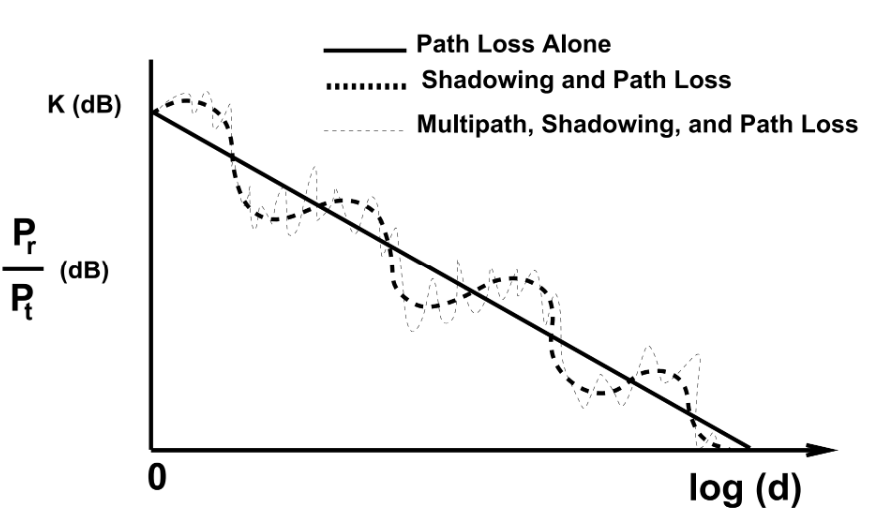
\includegraphics[width=0.6\textwidth]{fig/fig1.png}
		\caption{Path Loss, Shadowing og Multipath versus Distance.}
		\label{fig:path_loss_shadowing}
	\end{figure}
	
	\noindent Figur \ref{fig:path_loss_shadowing} viser forholdet mellem modtaget effekt (\(P_r\)) og transmitteret effekt (\(P_t\)) som en funktion af afstand (log(d)) i dB. Den fuldt optrukne linje repræsenterer effekten af path loss alene, den stiplede linje inkluderer effekterne af både path loss og shadowing, og den prikkede linje viser, hvordan multipath effekter kan skabe yderligere variationer. Figuren illustrerer, hvordan signalstyrken gradvist reduceres med øget afstand, og hvordan shadowing og multipath kan forårsage yderligere udsving i signalstyrken.	
	
	\section{Radio Wave Propagation}
	Den første forståelse af, hvordan radiobølger bevæger sig, stammer fra det banebrydende arbejde udført af James Clerk Maxwell i 1864. Maxwell udviklede teorien om elektromagnetiske bølger, som forudsagde, at radiobølger eksisterer. I 1887 beviste Heinrich Hertz eksperimentelt, at disse bølger faktisk eksisterer. Hertz mente dog, at radiobølger ikke havde nogen praktisk anvendelse, da han troede, at de ikke kunne bruges til at overføre stemme på grund af deres lave frekvens og dårlige udbredelse. Maxwells og Hertz' arbejde lagde grundlaget for radiokommunikation: i 1894 brugte Oliver Lodge disse principper til at skabe det første trådløse kommunikationssystem, selvom det kun kunne sende signaler op til 150 meter. I 1897 lykkedes det Guglielmo Marconi at sende et radiosignal fra Isle of Wight til en båd 18 miles væk, og i 1901 kunne hans system sende signaler over Atlanterhavet. Disse tidlige systemer brugte telegrafsignaler til at overføre information. I 1906 blev den første transmission af stemme og musik gennemført af Reginald Fessenden ved hjælp af amplitude modulation, hvilket omgåede de begrænsninger ved lave frekvenser, som Hertz havde påpeget, ved at flytte signalerne til en højere frekvens – en metode, der stadig anvendes i moderne trådløse systemer.
	\newline\newline\noindent
	Elektromagnetiske bølger bevæger sig gennem forskellige miljøer, hvor de kan reflekteres, spredes og brydes af forhindringer som vægge, terræn og bygninger. For at forstå disse processer i detaljer kan man bruge Maxwells ligninger, der kræver kendskab til de fysiske egenskaber af de objekter, som bølgerne interagerer med. Dette kan involvere komplekse beregninger af radar tværsnitsarealet (RCS) for store strukturer. Da disse beregninger ofte er svære og kræver data, som ikke altid er tilgængelige, benyttes der ofte tilnærmelsesmetoder til at beskrive signaludbredelse uden at skulle løse Maxwells ligninger.
	\newline\newline\noindent
	En af de mest anvendte tilnærmelser er strålesporingsteknikker. Disse metoder simplificerer udbredelsen af elektromagnetiske bølger ved at behandle bølgefronter som simple partikler. Modellen kan beskrive refleksioner og brydninger, men den ignorerer de mere komplekse spredningseffekter, som Maxwells ligninger forudsiger. En simpel strålesporingsmodel er tostrålemodellen, som beskriver udbredelsen, når der er én direkte vej mellem senderen og modtageren samt én reflekteret vej, typisk fra jorden. Denne model er god til at beskrive signaludbredelse langs motorveje, landeveje og over vand. Mere komplekse modeller overvejes også, hvor flere refleksioner, spredninger og brydninger inddrages. Mange miljøer kan dog ikke beskrives præcist med strålesporing alene. I disse tilfælde anvendes analytiske modeller baseret på empiriske målinger, og vi vil se på nogle af de mest almindelige empiriske modeller.
	\newline\newline\noindent
	Ofte er radiokanalens kompleksitet og variationer så store, at det er svært at opnå en nøjagtig deterministisk model. I sådanne tilfælde benyttes statistiske modeller ofte. Dæmpning forårsaget af hindringer som bygninger eller andre objekter beskrives typisk statistisk. Statistiske modeller bruges også til at beskrive den konstruktive og destruktive interferens fra mange multipath-komponenter. Disse modeller er mest præcise i miljøer med regelmæssige geometrier og ensartede dielektriske egenskaber. Indendørs miljøer har ofte mere uregelmæssige forhold end udendørs miljøer, da både geometri og dielektriske egenskaber kan variere betydeligt, afhængigt af om miljøet er en åben fabrik, kontor eller værksted. For sådanne miljøer er computerbaserede modelleringsværktøjer tilgængelige for at forudsige, hvordan signalerne udbredes.
	
	\section{Transmitterede og Modtagede Signaler}
	For at forstå modellerne for transmissions- og modtagesignaler i trådløse kommunikationssystemer, er det nødvendigt at starte med en beskrivelse af, hvad et signal er, og hvordan det påvirkes, når det passerer gennem en kommunikationskanal.
	
	\subsection{Transmitteret Signal}
	Vi modellerer det transmitterede signal \( s(t) \) som den reelle del af et komplekst signal:
	
	\[
	s(t) = \Re \{ u(t) e^{j2\pi f_c t} \}
	\]
	
	\noindent hvor \( u(t) \) er et komplekst basbåndssignal defineret som:
	
	\[
	u(t) = x(t) + jy(t)
	\]
	
	\noindent Her er \( x(t) \) den reelle komponent (in-phase) af basbåndssignalet, og \( y(t) \) er den imaginære komponent (kvadraturkomponenten). Disse komponenter har båndbredden \( B_u \) og effekten \( P_u \).
	
	\noindent Det komplekse basbåndssignal \( u(t) \) kan også skrives som:
	
	\[
	s(t) = x(t) \cos(2\pi f_c t) - y(t) \sin(2\pi f_c t)
	\]
	
	\noindent hvor \( f_c \) er bærefrekvensen.
	
	\noindent Signalet \( u(t) \) kaldes den \textit{komplekse kuvert} eller det \textit{komplekse lavpasækvivalente signal} for \( s(t) \). Dette navn kommer af, at \( |u(t)| \) repræsenterer amplituden, og argumentet af \( u(t) \) repræsenterer fasen af \( s(t) \).
	
	\subsection{Modtaget Signal}
	Det modtagede signal \( r(t) \) modelleres på samme måde:
	
	\[
	r(t) = \Re \{ v(t) e^{j2\pi f_c t} \}
	\]
	
	\noindent hvor \( v(t) \) er det komplekse basbåndssignal, der afhænger af den kanal, signalet transmitteres igennem. Hvis \( s(t) \) transmitteres gennem en tidsinvariant kanal, vil \( v(t) = u(t) * c(t) \), hvor \( c(t) \) er kanalens impulsrespons.
	
	\subsection{Doppler Effekt}
	Når modtageren bevæger sig i forhold til senderen, opstår en Doppler-forskydning, som resulterer i en frekvensskift \( f_D \) givet ved:
	
	\[
	f_D = \frac{1}{2\pi} \frac{\Delta \phi}{\Delta t} = \frac{v \cos \theta}{\lambda}
	\]
	
	\noindent hvor \( v \) er modtagerens hastighed mod senderen, \( \theta \) er vinklen mellem signalretningen og bevægelsesretningen, og \( \lambda = \frac{c}{f_c} \) er signalets bølgelængde.
	
	\subsection{Path Loss}
	Når et signal transmitteres gennem en given kanal, tabes noget af signalets effekt undervejs, hvilket kaldes \textit{path loss}. Dette tab kan udtrykkes som forholdet mellem den transmitterede effekt \( P_t \) og den modtagede effekt \( P_r \):
	
	\[
	P_L = \frac{P_t}{P_r}
	\]
	
	\noindent Dette kan også udtrykkes i dB som:
	
	\[
	P_L \, \text{dB} = 10 \log_{10} \left( \frac{P_t}{P_r} \right) \, \text{dB}
	\]
	
	\noindent Heraf kan man også definere \textit{path gain} \( P_G \) som:
	
	\[
	P_G = -P_L = 10 \log_{10} \left( \frac{P_r}{P_t} \right) \, \text{dB}
	\]
	
	\noindent Disse begreber bruges til at karakterisere, hvor meget signalstyrken reduceres eller forøges, når signalet bevæger sig gennem kommunikationskanalen.
	
	\section{Free-Space Path Loss og Doppler-effekt}
	
	\subsection{Free-Space Path Loss}
	Når et signal transmitteres gennem fri luft fra en sender til en modtager, og der ikke er nogen forhindringer mellem dem, beskriver vi transmissionen som værende over en line-of-sight (LOS) kanal. Det modtagne signal \( r(t) \) kan i dette tilfælde beskrives som:
	
	\[
	r(t) = \Re \left\{ \frac{\lambda \sqrt{G_t G_r} e^{-j2\pi d/\lambda}}{4\pi d} u(t) e^{j2\pi f_c t} \right\}
	\]
	
	\noindent hvor \( \lambda \) er signalets bølgelængde, \( G_t \) og \( G_r \) er forstærkningerne af henholdsvis sender- og modtagerantennerne, og \( d \) er afstanden mellem sender og modtager. Dette udtryk viser, at den modtagne signalstyrke falder omvendt proportionalt med kvadratet på afstanden \( d \), hvilket betyder, at signalet bliver svagere, jo længere det skal rejse.
	\newline\newline\noindent
	Forholdet mellem den modtagne og den transmitterede effekt kan derfor udtrykkes som:
	
	\[
	\frac{P_r}{P_t} = \left( \frac{\sqrt{G_t G_r} \lambda}{4\pi d} \right)^2
	\]
	
	\noindent Dette forhold kan også udtrykkes i dB som:
	
	\[
	P_L \text{ dB} = 10 \log_{10} \left(\frac{P_t}{P_r}\right) = -10 \log_{10} \left( \frac{G_t G_r \lambda^2}{(4\pi d)^2} \right)
	\]
	
	\subsection{Doppler-Effekt og Bevægelse}
	Når enten senderen eller modtageren bevæger sig, vil frekvensen af det modtagne signal blive forskudt på grund af Doppler-effekten. Dette kan beskrives som en ændring i frekvensen:
	
	\[
	f_D = \frac{v \cos \theta}{\lambda}
	\]
	
	\noindent hvor \( v \) er hastigheden af modtageren i forhold til senderen, og \( \theta \) er vinklen mellem modtagerens bevægelsesretning og signalets udbredelsesretning. 
	\newline\newline\noindent
	Figuren nedenfor illustrerer, hvordan en modtager i bevægelse i forhold til en stationær sender oplever en ændring i den modtagne frekvens:
	
	\begin{figure}[!h]
		\centering
		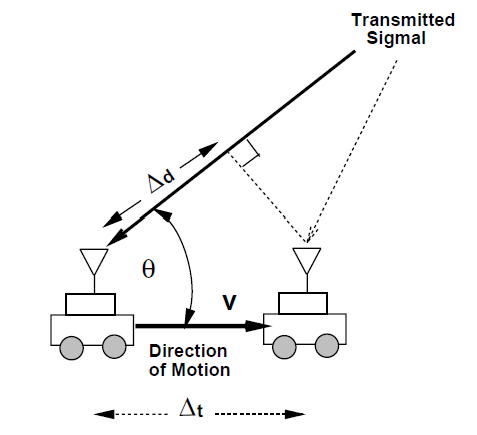
\includegraphics[width=0.4\textwidth]{fig/fig2.png} % Udskift med det faktiske billede i LaTeX-koden
		\caption{Doppler-effekt i en bevægende modtager.}
	\end{figure}

	\noindent Denne frekvensforskydning kan have en indflydelse på, hvordan signalet opfattes ved modtageren, og kan kombineres med overvejelser om path loss for at forudsige den faktiske modtagne signalstyrke i en dynamisk kommunikationsmiljø.
	
	\subsection{Eksempler}
	\subsubsection{Eksempel: Beregning af Path Loss i en Indendørs Trådløs LAN}
	Betragt et indendørs trådløst LAN med \( f_c = 900 \) MHz, en celleradius på 100 m, og ikke-retningsbestemte antenner. Vi kan beregne den nødvendige transmitterede effekt ved at bruge formlen for path loss og Doppler-effektens indflydelse:
	\[
	P_t = P_r \left( \frac{4\pi d}{\sqrt{G_t G_r} \lambda} \right)^2
	\]
	\noindent Ved at indsætte passende værdier for \( G_t \), \( G_r \), \( \lambda \), og \( d \), kan vi bestemme den nødvendige effekt for at sikre tilstrækkelig signalstyrke i hele cellen.
	
	\subsubsection{Eksempel 1: Beregning af Free-Space Path Loss}
	\textbf{Problem:} Betragt en trådløs kommunikationsforbindelse mellem en sender og en modtager, hvor senderen udsender en effekt på \( P_t = 1 \, \text{W} \) ved en frekvens på \( f_c = 2.4 \, \text{GHz} \). Afstanden mellem sender og modtager er \( d = 100 \, \text{m} \). Antag, at både senderen og modtageren bruger isotropiske antenner (dvs. \( G_t = G_r = 1 \)). Beregn den modtagne effekt \( P_r \).
	\newline\newline
	\noindent\textbf{Løsning:}
	\noindent
	Først beregner vi bølgelængden \( \lambda \):
	
	\[
	\lambda = \frac{c}{f_c} = \frac{3 \times 10^8 \, \text{m/s}}{2.4 \times 10^9 \, \text{Hz}} = 0.125 \, \text{m}
	\]
	
	\noindent Vi bruger formlen for forholdet mellem modtaget og transmitteret effekt:
	
	\[
	\frac{P_r}{P_t} = \left( \frac{\sqrt{G_t G_r} \lambda}{4\pi d} \right)^2
	\]
	
	\noindent Da \( G_t = G_r = 1 \):
	
	\[
	\frac{P_r}{1 \, \text{W}} = \left( \frac{0.125 \, \text{m}}{4\pi \times 100 \, \text{m}} \right)^2 = \left( \frac{0.125}{1256.64} \right)^2 = 9.89 \times 10^{-10}
	\]
	
	\noindent Den modtagne effekt \( P_r \) er således:
	
	\[
	P_r = 1 \, \text{W} \times 9.89 \times 10^{-10} = 9.89 \times 10^{-10} \, \text{W} = 0.989 \, \text{nW}
	\]
	
	\noindent I dBm:
	
	\[
	P_r \, \text{dBm} = 10 \log_{10} \left( 0.989 \times 10^{-9} \right) \approx -90.05 \, \text{dBm}
	\]
	
	\subsubsection{Eksempel 2: Beregning af Doppler-Skift}
	\textbf{Problem:} Antag, at en bil bevæger sig med en hastighed \( v = 30 \, \text{m/s} \) (svarende til ca. 108 km/t) mod en radiosender, der udsender ved en frekvens \( f_c = 900 \, \text{MHz} \). Beregn Doppler-forskydningen \( f_D \) hvis vinklen mellem bevægelsesretningen og signalretningen er \( \theta = 0^\circ \).
	\newline\newline\noindent
	\textbf{Løsning:}
	\noindent
	Doppler-forskydningen \( f_D \) beregnes ved hjælp af formlen:
	
	\[
	f_D = \frac{v \cos \theta}{\lambda}
	\]
	
	\noindent Først beregner vi bølgelængden \( \lambda \):
	
	\[
	\lambda = \frac{c}{f_c} = \frac{3 \times 10^8 \, \text{m/s}}{900 \times 10^6 \, \text{Hz}} = 0.333 \, \text{m}
	\]
	
	\noindent Da \( \theta = 0^\circ \) (dvs. \( \cos \theta = 1 \)):
	
	\[
	f_D = \frac{30 \, \text{m/s}}{0.333 \, \text{m}} = 90 \, \text{Hz}
	\]
	
	\noindent Doppler-forskydningen er således \( 90 \, \text{Hz} \), hvilket betyder, at den modtagne frekvens ved modtageren vil være \( f_c + f_D = 900.090 \, \text{MHz} \).
	
	
	\section{Ray Tracing}
	
	\noindent Forestil dig, at du kaster en bold i et rum fyldt med forskellige objekter som vægge, møbler og vinduer. Bolden vil ramme disse objekter og blive kastet tilbage i forskellige retninger. På samme måde, når et radiosignal (som en usynlig bølge) bliver sendt fra en sender i et bymiljø eller indenfor i en bygning, vil det støde på mange ting, der får signalet til at blive reflekteret, bøjet (diffracted), eller spredt. De ekstra signaler, som bliver skabt på denne måde, kaldes for \textit{multipath signal components}.
	\newline\newline\noindent
	Når disse multipath signaler når frem til modtageren, bliver de lagt sammen med det oprindelige signal. Dette kan resultere i, at det modtagne signal kan blive forvrænget (altså ændret i forhold til det oprindelige signal). 
	\begin{figure}[h]
		\centering
		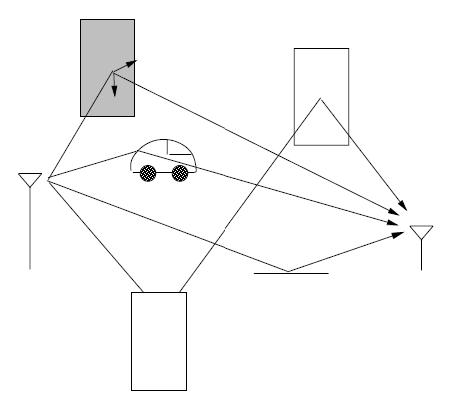
\includegraphics[width=0.6\textwidth]{fig/fig3.png}
		\caption{Reflected, Diffracted, and Scattered Wave Components.}
		\label{fig:ray_tracing}
	\end{figure}
	
	\noindent
	På billedet kan du se, hvordan et signal, der bliver sendt fra én kilde, kan reflekteres, bøjes, og spredes af objekter som bygninger, biler og vægge, før det når frem til modtageren.
	\newline\newline\noindent
	I \textit{ray tracing} antager vi, at der er et bestemt antal reflektorer (som de ting, signalet rammer) med kendte placeringer og egenskaber. Ved at bruge nogle ret avancerede ligninger, som Maxwell's ligninger, kan vi forudsige, hvordan signalet vil opføre sig, når det støder på disse objekter. Men disse beregninger kan være meget komplicerede og tage lang tid at udføre, så i praksis bruger vi ofte en forenklet metode, hvor vi behandler signalet som simple bølger, der bliver reflekteret, bøjet eller spredt.
	\newline\newline\noindent
	Denne metode fungerer bedst, når modtageren er langt væk fra den nærmeste genstand, og når genstandene, signalet rammer, er store sammenlignet med signalets bølgelængde.
	\newline\newline\noindent
	Hvis både senderen, modtageren og alle de ting, signalet rammer, ikke bevæger sig, så vil de \textit{multipath} signaler, der modtages, være ret stabile. Men hvis noget af det bevæger sig, vil disse signaler ændre sig over tid, og vi bliver nødt til at tage højde for det, når vi beregner, hvordan signalet vil se ud ved modtageren. I sådanne situationer bruger vi statistiske modeller for at forudsige, hvordan signalet vil opføre sig.
	\newline\newline\noindent
	De mest almindelige \textit{ray tracing} modeller inkluderer alle de reflekterede, bøjede og spredte signaler. Disse modeller bruger detaljerede oplysninger om både objekternes placering og deres fysiske egenskaber til at beregne, hvordan signalet vil opføre sig.
	\newline\newline\noindent
	Nogle populære computerprogrammer, som bruges til at planlægge trådløse systemer i både indendørs og udendørs miljøer, er \textit{Wireless Valley's SitePlanner®} og \textit{Marconi's Planet® EV}. Disse programmer kombinerer computergrafik med fotos eller tegninger af omgivelserne for at skabe et 3D-billede af miljøet.
	\newline\newline\noindent
	I praksis findes der flere forskellige \textit{ray tracing} modeller, som kan variere i kompleksitet:
	\begin{itemize}
		\item En simpel model, der forudsiger, hvordan et signal varierer på grund af en refleksion fra jorden.
		\item En mere avanceret model, der bruger op til ti refleksioner til at forudsige, hvordan et signal opfører sig langs en lige vej eller en gang.
		\item En generel model, der kan forudsige signaludbredelse i ethvert miljø.
	\end{itemize}
	Den enkle model kræver kun information om antennehøjder, mens de mere avancerede modeller også kræver detaljer om gadernes bredde i byområder eller gangenes bredde indendørs, samt om de objekter, der kan reflektere eller sprede signalet.
	
	\subsection{Two-Ray Model}
	
	\noindent Two-ray modellen bruges, når en enkelt refleksion fra jorden dominerer de multipath-effekter, som opstår, når signalet når frem til modtageren. I figur \ref{fig:two_ray_model} kan du se, hvordan signalet bevæger sig fra senderen til modtageren. Signalet opdeles i to dele: en direkte linje-of-sight (LOS) komponent, som er det direkte signal fra senderen, og en reflekteret komponent, som er signalet, der bliver reflekteret fra jorden.
	
	\begin{figure}[h]
		\centering
		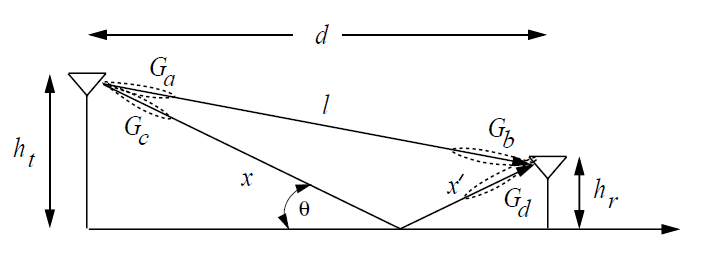
\includegraphics[width=0.8\textwidth]{fig/fig4.png}
		\caption{Two-Ray Model.}
		\label{fig:two_ray_model}
	\end{figure}
	
	\noindent
	Det modtagne LOS-signal beregnes ved hjælp af free-space propagation loss formlen, som vi så tidligere. Det reflekterede signal vises i figur \ref{fig:two_ray_model} som segmenterne \(x\) og \(x'\). Hvis vi ser bort fra effekten af overfladebølgedæmpning, så kan vi beregne det modtagne signal i two-ray modellen ved at kombinere LOS og det reflekterede signal:
	
	\[
	r_{2ray}(t) = \Re \left\{ \frac{\lambda}{4\pi} \left[ \frac{\sqrt{G_l} u(t) e^{-j2\pi l/\lambda}}{l} + \frac{R \sqrt{G_r} u(t - \tau) e^{-j2\pi(x+x')/\lambda}}{x + x'} \right] e^{j2\pi f_c t} \right\}
	\]
	
	\noindent
	Her er \( \tau = \frac{(x + x' - l)}{c} \) tidsforskellen mellem refleksionen og LOS-signalet, og \( \sqrt{G_l} = \sqrt{G_a G_b} \) er produktet af senderens og modtagerens antennediagrammer i LOS-retningen. \( R \) er refleksionskoefficienten, og \( \sqrt{G_r} = \sqrt{G_c G_d} \) er produktet af senderens og modtagerens antennediagrammer svarende til strålerne af længde \(x\) og \(x'\).
	
	\noindent
	Hvis det transmitterede signal er smalbåndet i forhold til tidsforskellen \( \tau \ll B_u^{-1} \), så kan \( u(t) \approx u(t - \tau) \). Med denne antagelse kan den modtagne effekt i two-ray modellen for smalbåndstransmission skrives som:
	
	\[
	P_r = P_t \left[ \frac{\lambda}{4\pi} \right]^2 \left| \frac{\sqrt{G_l}}{l} + \frac{R \sqrt{G_r} e^{-j\Delta \phi}}{x + x'} \right|^2
	\]
	
	\noindent
	Her er \( \Delta \phi = \frac{2\pi(x + x' - l)}{\lambda} \) faseskiftet mellem de to modtagne signaler. Ligning (2.12) er vist at være i god overensstemmelse med empiriske data.
	
	\noindent
	Når \( d \) (afstanden mellem sender og modtager) er meget større end \( h_t + h_r \), kan vi bruge en Taylor-serie tilnærmelse for at forenkle \( \Delta \phi \) til:
	
	\[
	\Delta \phi \approx \frac{4\pi h_t h_r}{\lambda d}
	\]
	
	\noindent
	Reflektionskoefficienten \( R \) kan beregnes ved hjælp af ligning (2.15):
	
	\[
	R = \frac{\sin \theta - Z}{\sin \theta + Z}
	\]
	
	\noindent
	Hvor \( Z \) afhænger af polariseringen af signalet, og \( \epsilon_r \) er materialets dielektriske konstant. For jord eller vejoverflader er \( \epsilon_r \) typisk omkring 15.
	
	\noindent
	I det asymptotiske tilfælde, hvor \( d \) er meget stor, vil den modtagne effekt falde med den fjerde potens af \( d \):
	
	\[
	P_r \approx P_t \left[ \frac{\lambda \sqrt{G_l}}{4\pi d} \right]^2 \left[ \frac{4\pi h_t h_r}{\lambda d} \right]^2
	\]
	
	\noindent
	I decibel (dB) kan den modtagne effekt skrives som:
	
	\[
	P_r \, \text{dBm} = P_t \, \text{dBm} + 10 \log_{10}(G_l) + 20 \log_{10}(h_t h_r) - 40 \log_{10}(d)
	\]
	
	\noindent
	Således, når \( d \) bliver meget stor, falder den modtagne effekt med fjerde potens af afstanden \( d \) og er uafhængig af bølgelængden \( \lambda \). Det modtagne signal bliver i dette tilfælde uafhængigt af \( \lambda \), da kombinationen af den direkte sti og det reflekterede signal ligner effekten af et antennediagram, og retningsbestemte antenner har en modtaget effekt, som ikke nødvendigvis falder med frekvensen.
	
	\begin{figure}[h]
		\centering
		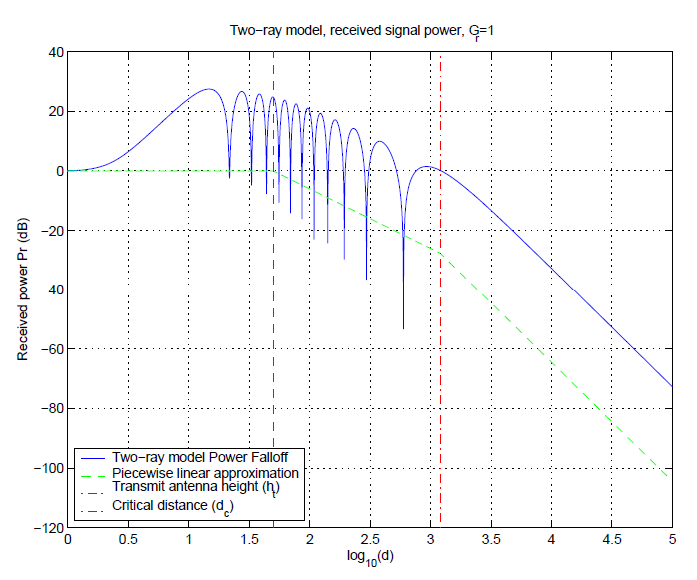
\includegraphics[width=0.8\textwidth]{fig/fig5.png}
		\caption{Received Power versus Distance for Two-Ray Model.}
		\label{fig:two_ray_falloff}
	\end{figure}
	
	\noindent
	Dette plot kan opdeles i tre segmenter. For små afstande (\( d < h_t \)) kombineres de to stråler konstruktivt, og path loss er nogenlunde flad. For moderate afstande, når \( d \) er proportional med \( \sqrt{d^2 + (h_t - h_r)^2} \), falder effekten med \( 1/(d^2 + h_t^2) \). For meget store afstande falder effekten med \( 1/d^4 \).
	
	\subsubsection{Kritisk Distance i Two-Ray Modellen}
	
	\noindent Den kritiske distance \( d_c \) i en two-ray model er afgørende for at bestemme, hvornår signalet fra den reflekterede stråle begynder at interferere signifikant med den direkte stråle. Denne distance kan beregnes ved hjælp af formlen:
	
	\[
	d_c = \frac{4h_t h_r}{\lambda}
	\]
	
	\noindent hvor:
	\begin{itemize}
		\item \( h_t \) og \( h_r \) er højderne på henholdsvis sender- og modtagerantennerne.
		\item \( \lambda \) er bølgelængden af signalet.
	\end{itemize}
	
	\noindent Når afstanden \( d \) mellem sender og modtager er større end \( d_c \), vil den modtagne signalstyrke falde hurtigt, hvilket kan have stor indflydelse på netværksplanlægning, især i byområder og indendørs miljøer.
	
	\subsubsection{Eksempel 2.2: Beregning af Kritisk Distance}
	
	\noindent I dette eksempel skal vi beregne den kritiske distance \( d_c \) for en bymæssig microcell (hvor \( h_t = 10 \) m og \( h_r = 3 \) m) og en indendørs microcell (hvor \( h_t = 3 \) m og \( h_r = 2 \) m) ved en frekvens \( f_c = 2 \) GHz.
	\newline\newline
	\noindent \textbf{Løsning:} Den kritiske distance \( d_c \) for en bymæssig microcell er 800 meter, mens den for en indendørs microcell er 160 meter. Disse afstande viser, at en celleradius på 800 m er for stor til et bymæssigt microcell system, hvor man typisk ønsker celler på omkring 100 m for at opretholde høj kapacitet. På samme måde er 160 m for stort til en indendørs microcell, hvor der typisk er mange vægge, som signalet skal passere igennem, hvilket kræver en mindre celleradius, omkring 10-20 m.
	
	\subsubsection{Eksempel 2.3: Beregning af Modtaget Effekt ved Forskellige Frekvenser}
	
	\noindent Beregn den modtagne effekt for en two-ray model, når sender- og modtagerhøjderne er \( h_t = 15 \) m og \( h_r = 2 \) m, og afstanden mellem dem er \( d = 500 \) m. Antag, at frekvensen \( f_c \) er henholdsvis 900 MHz og 2.4 GHz, og at antenneforstærkningen \( G_t = G_r = 1 \).
	
	\noindent \textbf{Løsning:} For 900 MHz beregnes den modtagne effekt ved:
	
	\[
	P_r \approx P_t \left[ \frac{\lambda}{4\pi d} \right]^2 \left[ \frac{4\pi h_t h_r}{\lambda d} \right]^2
	\]
	
	\noindent hvor \( \lambda = \frac{c}{f_c} = \frac{3 \times 10^8}{900 \times 10^6} = 0.333 \) m. Ved 2.4 GHz er \( \lambda = 0.125 \) m. Den modtagne effekt vil være højere ved 900 MHz end ved 2.4 GHz, fordi bølgelængden er længere, hvilket resulterer i mindre path loss.
	
	\subsubsection{Eksempel 2.4: Effekt af Antennehøjde på Modtaget Signalstyrke}
	
	\noindent Undersøg effekten af at øge højden på senderantennen \( h_t \) fra 10 m til 20 m, mens modtagerantennen forbliver på 2 m. Frekvensen er 1.8 GHz, og afstanden \( d \) mellem sender og modtager er 300 m. Beregn den relative ændring i modtaget signalstyrke.
	\newline\newline
	\noindent \textbf{Løsning:} Den relative ændring i modtaget effekt kan beregnes som forholdet mellem de modtagne effekter før og efter ændringen i \( h_t \):
	
	\[
	\frac{P_r'}{P_r} = \frac{(20 \times 2)}{(10 \times 2)} = 2
	\]
	
	\noindent Forøgelsen af senderantennens højde vil fordoble den modtagne effekt.
	
	\subsubsection{Eksempel 2.5: Effekt af Refleksionskoefficient på Signalstyrke}
	
	\noindent For en given two-ray model med \( h_t = 30 \) m, \( h_r = 10 \) m, \( d = 1 \) km, og en frekvens på 2 GHz, beregn den modtagne effekt, når refleksionskoefficienten \( R \) varierer mellem -1 og 0. Antag \( G_t = G_r = 1 \).
	\newline\newline
	\noindent \textbf{Løsning:} Ved \( R = -1 \) og \( R = 0 \) skal vi undersøge den modtagne effekt som en funktion af faseskiftet og refleksionskoefficienten. Ved \( R = -1 \) vil den modtagne effekt være minimal, da de to stråler vil interferere destruktivt. Ved \( R = 0 \) vil der ikke være nogen refleksion, og signalstyrken vil alene afhænge af LOS-komponenten.
	
	
	\subsection{Ten-Ray Model (Dielectric Canyon)}
	
	\noindent Ten-ray modellen, udviklet af Amitay, anvendes til at modellere signaludbredelse i urbane microcells, hvor gaderne er omgivet af bygninger på begge sider, og både sender- og modtagerantenner er placeret tæt på gadeniveau. Disse bygader fungerer som en dielektrisk kløft (canyon), hvor signalet udbredes. 
	\newline\newline
	\noindent I teorien kan et uendeligt antal stråler reflekteres fra bygningernes facader, inden de når frem til modtageren. Derudover kan strålerne også blive reflekteret fra bygninger bag senderen eller modtageren. Dog mister noget af signalenergien styrke ved hver refleksion, og signalveje, der involverer mere end tre refleksioner, kan generelt ignoreres. Når gadelayoutet er relativt lige, kan bagrefleksioner ofte også negligeres.
	\newline\newline
	\noindent Eksperimentelle data viser, at en model med ti refleksioner nøjagtigt kan repræsentere signaludbredelsen gennem denne dielektriske kløft. De ti stråler inkorporerer alle stier med én, to eller tre refleksioner, herunder:
	
	\begin{itemize}
		\item Linje-of-sight (LOS) stien,
		\item Jordreflekteret (GR) sti,
		\item Enkelt-væg (SW) reflekteret sti,
		\item Dobbelt-væg (DW) reflekteret sti,
		\item Tre-væg (TW) reflekteret sti,
		\item Væg-jord (WG) reflekteret sti,
		\item og Væg-væg (GW) reflekteret sti.
	\end{itemize}
	
	\noindent Figur \ref{fig:ten_ray_model} viser et overblik over disse stier i ten-ray modellen.
	
	\begin{figure}[h]
		\centering
		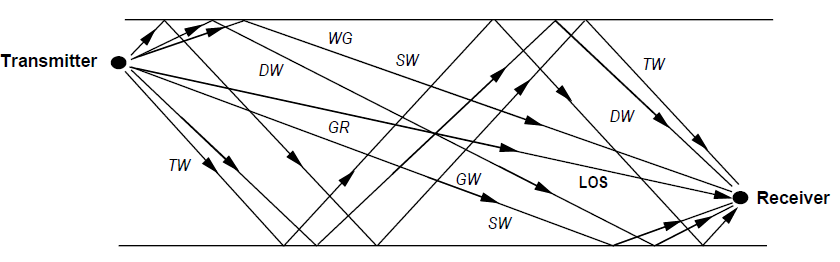
\includegraphics[width=0.8\textwidth]{fig/fig6.png}
		\caption{Overhead View of the Ten-Ray Model.}
		\label{fig:ten_ray_model}
	\end{figure}
	
	\noindent For ten-ray modellen kan det modtagne signal udtrykkes som:
	
	\[
	r_{10ray}(t) = \Re \left\{ \frac{\lambda}{4\pi} \left[ \frac{\sqrt{G_l} u(t) e^{-j2\pi l/\lambda}}{l} + \sum_{i=1}^{9} \frac{R_i \sqrt{G_{xi}} u(t - \tau_i) e^{-j2\pi x_i/\lambda}}{x_i} \right] e^{j2\pi f_c t} \right\}
	\]
	
	\noindent Her er \( x_i \) længden af stien for den i'te reflekterede stråle, \( \tau_i = \frac{(x_i - l)}{c} \) er tidsforsinkelsen mellem LOS-signalet og den i'te refleksion, og \( \sqrt{G_{xi}} \) er produktet af sender- og modtagerantennens gevinst i den i'te retning. For hver refleksionssti er koefficienten \( R_i \) enten en enkelt refleksionskoefficient (beregnet ved hjælp af ligning (2.15)) eller, hvis stien involverer flere refleksioner, produktet af refleksionskoefficienterne for hver refleksion. 
	\newline\newline
	\noindent Ligning for refleksionskoefficienten \( R \) er:
	
	\[
	R = \frac{\sin \theta - Z}{\sin \theta + Z}
	\]
	
	\noindent Hvor:
	
	\[
	Z = \begin{cases} 
		\sqrt{\epsilon_r - \cos^2\theta}/\epsilon_r & \text{for vertikal polarisering} \\
		\sqrt{\epsilon_r - \cos^2\theta} & \text{for horisontal polarisering}
	\end{cases}
	\]
	
	\noindent Her er \(\epsilon_r\) jordens eller vejens dielektriske konstant, som typisk er omkring 15.
	\newline\newline
	\noindent Den modtagne effekt kan udtrykkes som:
	
	\[
	P_r = P_t \left[ \frac{\lambda}{4\pi} \right]^2 \left| \frac{\sqrt{G_l}}{l} + \sum_{i=1}^{9} \frac{R_i \sqrt{G_{xi}} e^{-j\Delta \phi_i}}{x_i} \right|^2
	\]
	
	\noindent Hvor \( \Delta \phi_i = \frac{2\pi(x_i - l)}{\lambda} \) er faseskiftet mellem den i'te reflekterede stråle og LOS-strålen. 
	\newline\newline
	\noindent Power falloff i både ten-ray modellen og empiriske data viser, at signalstyrken falder proportionalt med \( d^{-2} \), selv ved relativt store afstande. Denne dæmpning er relativt ufølsom over for højden på senderantennen. Den kombinerede effekt af multipath-strålerne, som falder som \( d^{-2} \), og den ground-reflekterede stråle (som falder som \( d^{-4} \) i two-ray modellen) resulterer i et total power falloff med afstand, der er proportional med \( d^{-\gamma} \), hvor \( \gamma \) typisk ligger mellem to og seks.
	
	\subsubsection{Eksempel 2.6: Beregning af Modtaget Effekt for SW og DW Stier}
	
	\noindent Antag en Ten-Ray model, hvor sender- og modtagerhøjderne er \( h_t = 10 \) m og \( h_r = 2 \) m, og afstanden mellem dem er \( d = 100 \) m. Beregn den modtagne effekt for enkelt-væg (SW) og dobbelt-væg (DW) reflekterede stier ved en frekvens \( f_c = 2.4 \) GHz.	
	\newline\newline
	\noindent \textbf{Løsning:} Først beregner vi bølgelængden \( \lambda \) for frekvensen \( f_c = 2.4 \) GHz:
	
	\[
	\lambda = \frac{c}{f_c} = \frac{3 \times 10^8 \text{ m/s}}{2.4 \times 10^9 \text{ Hz}} = 0.125 \text{ m}
	\]
	
	\noindent For SW-stien (enkelt-væg) beregnes den modtagne effekt ved hjælp af:
	
	\[
	P_r \approx P_t \left[ \frac{0.125 \text{ m}}{4\pi \times 100 \text{ m}} \right]^2 \left| \frac{R_{SW} \sqrt{G_{x_{SW}}} e^{-j\Delta \phi_{SW}}}{x_{SW}} \right|^2
	\]
	
	\noindent For DW-stien (dobbelt-væg) beregnes den modtagne effekt ved at tage hensyn til dobbeltrefleksion:
	
	\[
	P_r \approx P_t \left[ \frac{0.125 \text{ m}}{4\pi \times 100 \text{ m}} \right]^2 \left| \frac{R_{DW} \sqrt{G_{x_{DW}}} e^{-j\Delta \phi_{DW}}}{x_{DW}} \right|^2
	\]
	
	\noindent Hvis vi antager, at \( x_{SW} = 120 \text{ m} \) og \( x_{DW} = 140 \text{ m} \), samt typiske værdier for refleksionskoefficienterne, kan vi beregne den samlede modtagne effekt som summen af bidragene fra begge stier.
	
	\subsubsection{Eksempel 2.7: Effekt af Dielektrisk Konstant på Modtaget Signal}
	
	\noindent Undersøg effekten af at variere den dielektriske konstant \( \epsilon_r \) fra 10 til 20 på den modtagne effekt i en Ten-Ray model ved en frekvens \( f_c = 900 \) MHz. Sender- og modtagerhøjderne er \( h_t = 15 \) m og \( h_r = 2 \) m, og afstanden \( d \) er 200 m.
	\newline\newline
	\noindent \textbf{Løsning:} Bølgelængden \( \lambda \) for frekvensen \( f_c = 900 \) MHz er:
	
	\[
	\lambda = \frac{c}{f_c} = \frac{3 \times 10^8 \text{ m/s}}{900 \times 10^6 \text{ Hz}} = 0.333 \text{ m}
	\]
	
	\noindent Reflektionskoefficienten \( R \) beregnes for hver værdi af \( \epsilon_r \) ved hjælp af ligning 2.15:
	
	\[
	R = \frac{\sin \theta - Z}{\sin \theta + Z}
	\]
	
	\noindent For \( \epsilon_r = 10 \) og \( \epsilon_r = 20 \), vi bruger værdierne til at beregne \( Z \) og derefter \( R \). Forøgelsen af \( \epsilon_r \) vil generelt reducere refleksionskoefficienten, hvilket resulterer i en lavere modtaget effekt. Den eksakte ændring i modtaget effekt kan beregnes ved at substituere de nye værdier for \( R \) i formlen for \( P_r \).
	
	\subsubsection{Eksempel 2.8: Beregning af Modtaget Effekt ved Forskellige Senderhøjder}
	For en Ten-Ray model, hvor \( h_t \) varierer mellem 5 m og 20 m, beregn den modtagne effekt ved en fast modtagerhøjde \( h_r = 3 \) m og en afstand \( d = 150 \) m. Frekvensen er \( f_c = 1.8 \) GHz.
	\newline\newline
	\noindent \textbf{Løsning:} Bølgelængden \( \lambda \) for frekvensen \( f_c = 1.8 \) GHz er:
	
	\[
	\lambda = \frac{c}{f_c} = \frac{3 \times 10^8 \text{ m/s}}{1.8 \times 10^9 \text{ Hz}} = 0.167 \text{ m}
	\]
	
	\noindent Den modtagne effekt afhænger af senderhøjden \( h_t \), da den påvirker signalets vej og de involverede refleksioner. Beregn den modtagne effekt for hver værdi af \( h_t \) ved at substituere ind i formlen for \( P_r \) og observere, hvordan effekten ændres med senderhøjden. For eksempel, hvis \( h_t \) stiger fra 5 m til 20 m, vil den modtagne effekt ændre sig markant, især på grund af ændringerne i faseskift og refleksioner.
	
	
	
	\subsection{General Ray Tracing (GRT)}
	General Ray Tracing (GRT) er en teknik, der anvendes til at forudsige signalstyrke og delay spread for ethvert bygningkonfiguration og antenneplacering. Denne metode er afhængig af en bygningdatabase, som indeholder information om højde, placering og dielektriske egenskaber af bygninger samt placeringen af transmitter- og receiverantennerne i forhold til bygningerne. Da denne information er site-specific, anvendes GRT-modellen ikke til at udlede generelle teorier om systemperformance og layout, men derimod til at forklare de grundlæggende mekanismer i urban signaludbredelse. Modellen bruges til at opnå information om delay og signalstyrke for en specifik transmitter- og receiver-konfiguration i et givet miljø.
	\newline\newline\noindent GRT-metoden bruger geometrical optics til at spore udbredelsen af Line-of-Sight (LOS) og reflekterede signal komponenter, samt signaler fra bygning diffraction og diffus scattering. Der er ingen begrænsning på antallet af multipath komponenter, der kan indregnes på en given modtager lokation. Styrken af hver komponent bestemmes eksplicit ud fra bygningernes placeringer og deres dielektriske egenskaber. I almindelighed giver LOS- og reflekterede stier de dominerende komponenter af det modtagne signal, da diffraction og scattering tab normalt er høje. Men i områder tæt på LOS og refleksionsstrålerne kan disse andre multipath-komponenter dominere.
	\subsubsection{Eksempel 1: Beregning af Signaltab gennem Bygninger}
	\noindent Antag, at vi har en bygning med en dielektrisk konstant \( \epsilon_r = 4 \). Et signal med en frekvens på 2 GHz skal passere gennem en 30 meter lang bygning. Beregn signaltabet ved hjælp af GRT-modellen.
	\newline\newline
	\noindent \textbf{Løsning:}
	\begin{enumerate}
		\item \textbf{Frekvens og Bølgelængde:} Frekvens \( f_c = 2 \) GHz. Bølgelængde \( \lambda = \frac{c}{f_c} = \frac{3 \times 10^8 \text{ m/s}}{2 \times 10^9 \text{ Hz}} = 0.15 \text{ meter} \).
		\item \textbf{Signaltab pr. meter:} Antag, at tabet pr. meter \( L_b \) er 0,5 dB/m. 
		\item \textbf{Samlet signaltab:} 
		\[
		L_{\text{total}} = L_b \times \text{distance} = 0.5 \text{ dB/m} \times 30 \text{ m} = 15 \text{ dB}
		\]
		\item \textbf{Resultat:} Det totale signaltab gennem bygningen er 15 dB.
	\end{enumerate}
	
	\subsubsection{Eksempel 2: Beregning af Refleksion fra en Bygning}
	\noindent En signalstråle reflekteres fra en glasbygning 50 meter væk fra en sender. Beregn signalstyrken ved en modtager 100 meter væk fra senderen efter refleksion.
	\newline\newline
	\noindent \textbf{Løsning:}
	\begin{enumerate}
		\item \textbf{Reflektionskoefficient:} Antag, at refleksionskoefficienten \( R \) for glas er 0.7.
		\item \textbf{Fri rums tab:}
		\[
		L_f = 20 \log_{10}\left(\frac{4\pi \times 100 \text{ m}}{\lambda}\right) \text{ dB}
		\]
		\[
		\lambda = 0.15 \text{ meter}, \quad L_f \approx 51.5 \text{ dB}
		\]
		\item \textbf{Total signaltab:}
		\[
		L_{\text{total}} = L_f + 10 \log_{10}(R) = 51.5 \text{ dB} - 1.55 \text{ dB} = 49.95 \text{ dB}
		\]
		\item \textbf{Resultat:} Den modtagne signalstyrke er reduceret med ca. 49.95 dB.
	\end{enumerate}
	
	\subsubsection{Eksempel 3: Brug af GRT til Antenneplacering}
	\noindent En mobiloperatør skal placere en antenne i en by for optimal dækning. GRT bruges til at simulere signaludbredelsen fra forskellige placeringer.
	\newline\newline
	\noindent \textbf{Løsning:}
	\begin{enumerate}
		\item \textbf{Bygningsdata:} Indlæs bygningsdata som højde, placering og dielektriske egenskaber.
		\item \textbf{Signaludbredelse:} Brug GRT til at simulere signaludbredelsen fra forskellige antenneplaceringer.
		\item \textbf{Analyse:} Sammenlign resultatet af hver placering og vælg den, der giver den bedste dækning og signalstyrke.
	\end{enumerate}
	\subsection{Knife-Edge Diffraction} Udbredelsesmodellen for LOS- og reflekterede stier blev forklaret i det forrige afsnit. Diffraction opstår, når det transmitterede signal "bøjes rundt om" et objekt på dets vej til modtageren, som vist i Figur \ref{fig:knife_edge_diffraction}. Diffraction er resultatet af mange fænomen, herunder jordens overflade, ujævnt terræn, bygninger, eller forhindringer, der blokerer LOS-path mellem transmitter og receiver.
	\newline\newline\noindent Knivkant diffraction modellen (Knife-Edge Diffraction Model) bruges ofte til at modellere diffraction, fordi den er enkel at anvende og kan levere en præcis approximation, selvom det ikke er den mest generelle model. I denne model antages det, at objektet, der forårsager diffractionen, har en kileform, hvilket er almindeligt for gadehjørner. Knivkant diffraction modellen forudsiger, at det diffrakterede signal rejser en ekstra distance \( d + d' \), hvilket resulterer i et faseskift på \( \Delta \phi = 2\pi(d + d')/\lambda \). Geometrien i Figur \ref{fig:knife_edge_diffraction} indikerer, at for \( h \) lille i forhold til \( d \) og \( d' \), skal signalet rejse en ekstra distance relativt til LOS-path på cirka:

	\[
	\Delta d = \frac{h^2 d + d'}{2 dd'}
	\]
	og det tilsvarende faseskift relativt til LOS-path er cirka:

	\[
	\Delta \phi = \frac{2\pi \Delta d}{\lambda} = \frac{\pi}{2} v^2
	\]
	hvor
	
	\[
	v = h \frac{\sqrt{2(d+d')}}{\lambda \cdot d \cdot d'}
	\]
	\noindent Dette kaldes Fresnel-Kirchhoff diffraction parameteren. De tilhørende tab, kaldet knife-edge diffraction loss, er en funktion af \( v \). Approximationer for knife-edge diffraction loss i dB relativt til LOS-path loss er givet af:

	\[
	L(v) \text{ dB} = \left\{
	\begin{array}{ll}
		20 \log_{10}[0.5 - 0.62v] & -0.8 \leq v < 0 \\
		20 \log_{10}[0.5e^{-0.95v}] & 0 \leq v < 1 \\
		20 \log_{10}[0.4 - \sqrt{0.1184 - (0.38 - 0.1v)^2}] & 1 \leq v < 2.4 \\
		20 \log_{10}[0.225/v] & v \geq 2.4
	\end{array}
	\right.
	\]
	\noindent Knife-edge diffraction modellen giver følgende formel for det modtagne diffrakterede signal:

	\[
	r(t) = \Re \left\{ L(v) \sqrt{G_d} u(t - \tau) e^{-j2\pi(d+d')/\lambda} e^{j2\pi f_c t} \right\}
	\]
	\noindent hvor \( \sqrt{G_d} \) er antenneforstærkningen og \( \tau = \Delta d / c \) er forsinkelsen forbundet med det diffrakterede signal relativt til LOS-path.
	\begin{figure}[h]
		\centering
		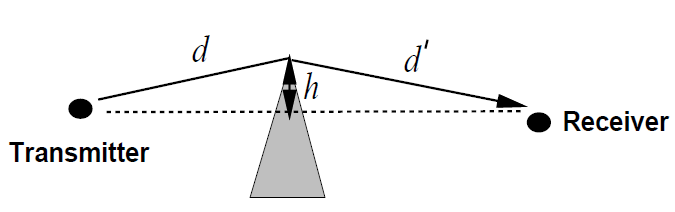
\includegraphics[width=0.8\textwidth]{fig/fig7.png}
		\caption{Knife-Edge Diffraction.}
		\label{fig:knife_edge_diffraction}
	\end{figure}
	\subsubsection{Eksempel 4: Beregning af Faseskift ved Knife-Edge Diffraction}
	\noindent Et signal diffrakteres omkring et hjørne med en højde \( h = 10 \) meter. Afstanden til modtageren er \( d = 100 \) meter, og til den anden side af hjørnet \( d' = 50 \) meter. Frekvensen er 2.4 GHz. Beregn faseskiftet \( \Delta \phi \).
	\newline\newline
	\noindent \textbf{Løsning:}
	\begin{enumerate}
		\item \textbf{Beregning af bølgelængde:} 
		\[
		\lambda = \frac{c}{f_c} = \frac{3 \times 10^8}{2.4 \times 10^9} = 0.125 \text{ meter}
		\]
		\item \textbf{Beregn \( v \):}
		\[
		v = h \frac{\sqrt{2(d+d')}}{\lambda \cdot d \cdot d'} = 10 \cdot \frac{\sqrt{2 \cdot (100 + 50)}}{0.125 \cdot 100 \cdot 50} = 0.8
		\]
		\item \textbf{Beregn faseskift \( \Delta \phi \):}
		\[
		\Delta \phi = \frac{\pi}{2}v^2 = \frac{\pi}{2}(0.8)^2 = 1.005 \text{ rad}
		\]
		\item \textbf{Resultat:} Faseskiftet er ca. 1.005 radianer.
	\end{enumerate}
	
	\subsubsection{Eksempel 5: Beregning af Diffraction Tab}
	\noindent Antag, at \( v = 1.5 \) for en given knife-edge diffraction. Beregn diffraction tabet \( L(v) \) i dB.
	\newline\newline
	\noindent \textbf{Løsning:}
	\begin{enumerate}
		\item \textbf{Beregn diffraction tabet:}
		\[
		L(v) \text{ dB} = 20 \log_{10}[0.4 - \sqrt{0.1184 - (0.38 - 0.1 \cdot 1.5)^2}]
		\]
		\item \textbf{Resultat:} Diffraction tabet er ca. -12 dB.
	\end{enumerate}
	
	\subsubsection{Eksempel 6: Modtaget Signalstyrke efter Diffraction}
	\noindent Et signal med en styrke på 0 dBm diffrakteres omkring et objekt med \( v = 2 \). Beregn den modtagne signalstyrke.
	\newline\newline
	\noindent \textbf{Løsning:}
	\begin{enumerate}
		\item \textbf{Beregn diffraction tabet:} 
		\[
		L(v) \text{ dB} = 20 \log_{10}[0.225/v] = 20 \log_{10}[0.225/2] = -20 \text{ dB}
		\]
		\item \textbf{Modtaget signalstyrke:} 
		\[
		P_r = 0 \text{ dBm} - 20 \text{ dB} = -20 \text{ dBm}
		\]
		\item \textbf{Resultat:} Den modtagne signalstyrke er -20 dBm.
	\end{enumerate}
	
	\subsection{Scattering}
	\noindent Foruden diffrakterede stråler kan der også være stråler, der er diffrakterede flere gange eller stråler, der både er reflekterede og diffrakterede. Modeller findes for at inkludere alle mulige permutationer af refleksion og diffraction, men attenuationen af de tilsvarende signal komponenter er generelt så stor, at disse komponenter er negligibelt i forhold til støj. Diffraction modeller kan også specialiseres til et givet miljø. For eksempel blev en model for diffraction fra bygninger og tage i cellular systems udviklet af Walfisch og Bertoni. 
	\newline\newline\noindent En scattered stråle, vist i Figur \ref{fig:scattering}, har et path loss proportionalt med produktet af \( s \) og \( s' \). Denne multiplicative afhængighed skyldes det ekstra spredningstab, som strålen oplever efter spredning. Det modtagne signal på grund af en scattered stråle er givet af den bistatiske radar ligning:

	\[
	r(t) = \Re \left\{ u(t - \tau) \frac{\lambda \sqrt{G_s} \sigma e^{-j2\pi(s+s')/\lambda}}{(4\pi)^{3/2}ss'} e^{j2\pi f_c t} \right\}
	\]
	\noindent hvor \( \tau = (s + s' - l)/c \) er forsinkelsen forbundet med den spredte stråle, \( \sigma \) er radar cross section for scatteren, og \( G_s \) er antenneforstærkning. Denne model antager, at signalet udbreder sig fra transmitter til scatterer baseret på free space propagation og derefter reemitteres af scatteren med transmit power \( \sigma \) til at estimere den modtagne effekt ved scattereren.
	
	\begin{figure}[!h]
		\centering
		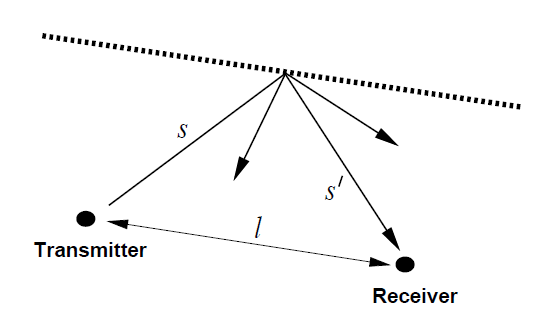
\includegraphics[width=0.6\textwidth]{fig/fig8.png}
		\caption{Scattering.}
		\label{fig:scattering}
	\end{figure}

	\subsubsection{Eksempel 7: Beregning af Spredt Signalstyrke}
	\noindent Et signal spredes af en lille metalgenstand med en radar cross section \( \sigma = 0.1 \) kvadratmeter. Afstanden mellem senderen og objektet er 50 meter, og mellem objektet og modtageren er 70 meter. Frekvensen er 1.8 GHz. Beregn den modtagne signalstyrke.
	\noindent \textbf{Løsning:}
	\begin{enumerate}
		\item \textbf{Beregning af bølgelængde:} 
		\[
		\lambda = \frac{c}{f_c} = \frac{3 \times 10^8}{1.8 \times 10^9} \approx 0.167 \text{ meter}
		\]
		\item \textbf{Beregn spredt signalstyrke:}
		\[
		P_r = P_t \cdot \frac{\lambda \sqrt{G_s} \sigma}{(4\pi)^{3/2}ss'} 
		\]
		\[
		s = 50 \text{ meter}, \quad s' = 70 \text{ meter}, \quad G_s = 1, \quad \sigma = 0.1
		\]
		\[
		P_r = P_t \cdot \frac{0.167 \times 0.1}{(4\pi)^{3/2} \times 50 \times 70} \approx P_t \cdot 1.59 \times 10^{-8}
		\]
		\item \textbf{Resultat:} Den modtagne signalstyrke vil være meget lav, ca. \( P_t \times 1.59 \times 10^{-8} \).
	\end{enumerate}
	
	\subsubsection{Eksempel 8: Effekt af Antennens Gain på Spredt Signal}
	\noindent Hvis antennen har en gain \( G_s = 3 \) ved en frekvens på 2.4 GHz, og signalet spredes af et objekt 100 meter væk, beregn effekten af denne gain på den modtagne signalstyrke.
	
	\noindent \textbf{Løsning:}
	\begin{enumerate}
		\item \textbf{Beregning af spredt signalstyrke:} 
		\[
		P_r = P_t \cdot \frac{\lambda \sqrt{G_s} \sigma}{(4\pi)^{3/2}ss'}
		\]
		\[
		G_s = 3, \quad s = 100 \text{ meter}, \quad s' = 100 \text{ meter}, \quad \sigma = 0.1
		\]
		\[
		P_r = P_t \cdot \frac{0.125 \times \sqrt{3} \times 0.1}{(4\pi)^{3/2} \times 100 \times 100}
		\]
		\item \textbf{Resultat:} Den modtagne signalstyrke stiger i forhold til \( G_s = 1 \).
	\end{enumerate}
	
	\subsubsection{Eksempel 9: Beregning af Spredningstab}
	\noindent Beregn spredningstab, når et signal med \( P_t = 10 \) dBm reflekteres og spredes af et objekt 70 meter væk fra både sender og modtager.
	
	\noindent \textbf{Løsning:}
	\begin{enumerate}
		\item \textbf{Beregning af bølgelængde:}
		\[
		\lambda = 0.167 \text{ meter}, \quad s = s' = 70 \text{ meter}, \quad \sigma = 0.05
		\]
		\item \textbf{Spredt signalstyrke:}
		\[
		P_r = 10 \text{ dBm} + 10 \log_{10}\left( \frac{0.167 \times 0.05}{(4\pi)^{3/2} \times 70 \times 70} \right)
		\]
		\item \textbf{Resultat:} 
		\[
		P_r \approx -60 \text{ dBm}
		\]
	\end{enumerate}

	\subsection{Local Mean Received Power}
	The path loss beregnet fra alle ray tracing modeller er forbundet med en fast transmitter og receiver lokation. Derudover kan ray tracing bruges til at beregne den lokale gennemsnitlige
	modtagne effekt \( P_r \) i nærheden af en given receiver lokation ved at tilføje den kvadrerede størrelse af alle de modtagne stråler. Dette har effekten af at udglatte lokale spatial variationer på grund af faseændringer rundt omkring en given lokation. Local mean received power er en god indikator for link quality og bruges ofte i cellular systems til power control og handoff.
	
	\subsection{Local Mean Received Power} Det path loss, som beregnes fra alle ray tracing-modeller, er knyttet til en fast position af både sender og modtager. Når man arbejder med trådløse signaler, er det dog også vigtigt at
	forstå, hvordan den modtagne effekt varierer i et lokalt område omkring modtageren. Dette kan gøres ved at beregne den \textit{local mean received power} \( \overline{P_r} \).
	\newline\newline
	\textit{Local mean received power} er den gennemsnitlige værdi af den modtagne effekt i et lille område omkring modtageren. For at beregne denne størrelse, tager man højde for alle de forskellige signalveje (rays), der når frem til modtageren. Hver af disse signaler kan have en forskellig amplitude og fase, hvilket betyder, at når man summerer bidragene fra alle signalerne, skal man først kvadrere hver signals amplitude, inden man summerer dem. Denne proces udjævner lokale rumlige variationer, som skyldes faseændringer omkring den specifikke position.
	\newline\newline
	Den \textit{local mean received power} \( \overline{P_r} \) er en god indikator for kvaliteten af en trådløs forbindelse og anvendes ofte i cellulære systemer til funktioner som power control og handoff.
	
	\section{Empiriske Path Loss Modeller}
	Empiriske path loss modeller bruges til at forudsige signalstyrke i komplekse udbredelsesmiljøer, hvor simple modeller som free-space path loss eller ray tracing ikke er tilstrækkelige. Disse modeller er baseret på faktiske målinger af signaludbredelse i specifikke miljøer, såsom store byområder (\textit{urban macrocells}), mindre byområder (\textit{urban microcells}) og indendørs omgivelser. Modellerne anvender typisk data fra bestemte geografiske områder eller bygningstyper og giver os mulighed for at vurdere signalstyrken på forskellige afstande og frekvenser.
	
	\subsection{The Okumura Model}
	Okumura-modellen er en af de mest anvendte modeller til signalforudsigelse i store byområder. Modellen er gældende over afstande fra 1 til 100 km og frekvensområder fra 150 til 1500 MHz. Den er baseret på omfattende målinger af signaludbredelse fra basestationer til mobile enheder i Tokyo, Japan. Modellen estimerer den mediane attenuation i forhold til free space udbredelse. Formlen for path loss ved en afstand \(d\) er:
	
	\[
	P_L(d) = L(f_c, d) + A_{\text{mu}}(f_c, d) - G(h_t) - G(h_r) - G_{\text{AREA}}
	\]
	
	Her er:
	\begin{itemize}
		\item \( L(f_c, d) \): free space path loss ved afstand \(d\) og frekvens \(f_c\),
		\item \( A_{\text{mu}}(f_c, d) \): den mediane attenuation,
		\item \( G(h_t) \): gevinst fra senderantennens højde, beregnet som:
		\[
		G(h_t) = 20\log_{10}\left(\frac{h_t}{200}\right), \quad 30m < h_t < 1000m
		\]
		\item \( G(h_r) \): gevinst fra modtagerantennens højde, beregnet som:
		\[
		G(h_r) = \left\{
		\begin{array}{ll}
			10\log_{10}\left(\frac{h_r}{3}\right), & h_r \leq 3m \\
			20\log_{10}\left(\frac{h_r}{3}\right), & 3m < h_r \leq 10m 
		\end{array}
		\right.
		\]
		\item \( G_{\text{AREA}} \): gevinst afhængig af områdets karakteristika.
	\end{itemize}
	
	\subsection{The Hata Model}
	Hata-modellen er en videreudvikling af Okumura-modellen og bruges til at forenkle beregningen af path loss med en lukket formel. Denne model dækker stort set samme frekvensområde som Okumura-modellen og bruges især i byområder. Formlen for path loss i byområder er:
	
	\[
	P_L(d) = 69.55 + 26.16 \log_{10}(f_c) - 13.82 \log_{10}(h_t) - a(h_r) + \left( 44.9 - 6.55 \log_{10}(h_t) \right) \log_{10}(d)
	\]
	
	Her er \( a(h_r) \) en korrektion for modtagerantennens højde afhængigt af størrelsen af byområdet, beregnet som:
	
	\[
	a(h_r) = \left\{
	\begin{array}{ll}
		(1.1 \log_{10}(f_c) - 0.7)h_r - (1.56 \log_{10}(f_c) - 0.8) \text{ dB}, & \text{for små til mellemstore byer,} \\
		3.2(\log_{10}(11.75h_r))^2 - 4.97 \text{ dB}, & \text{for større byer,} \\
	\end{array}
	\right.
	\]
	
	\subsection{COST 231 Udvidelse til Hata Modellen}
	COST 231 er en udvidelse af Hata-modellen, som dækker højere frekvenser (op til 2 GHz) og bruges i byområder med mellemstore byer og forstæder. Formlen for path loss er:
	
	\[
	P_L(d) = 46.3 + 33.9 \log_{10}(f_c) - 13.82 \log_{10}(h_t) - a(h_r) + \left( 44.9 - 6.55 \log_{10}(h_t) \right) \log_{10}(d) + C_M
	\]
	
	Hvor \( C_M \) er en konstant på 0 dB for byområder og 3 dB for forstæder.
	
	\subsection{Piecewise Linear (Multi-Slope) Model}
	
	En almindelig empirisk metode til modellering af \textit{path loss} i udendørs \textit{microcells} og indendørs kanaler er \textit{piecewise linear} modellen, som illustrerer dB-tab som funktion af log-afstanden. Denne tilgang er illustreret i Figur \ref{fig:piecewise_linear_model}, hvor punkterne repræsenterer hypotetiske empiriske målinger, og den stykvis lineære model repræsenterer en approximation til disse målinger. En \textit{piecewise linear} model med \(N\) segmenter skal specificere \(N-1\) brudpunkter \(d_1, d_2, \ldots, d_{N-1}\) og hældningerne svarende til hvert segment \(s_1, s_2, \ldots, s_N\). Forskellige metoder kan bruges til at bestemme antallet og placeringen af brudpunkter i modellen. Når disse er fastlagt, kan hældningerne svarende til hvert segment opnås ved lineær regression.
	
	\begin{figure}[h]
		\centering
		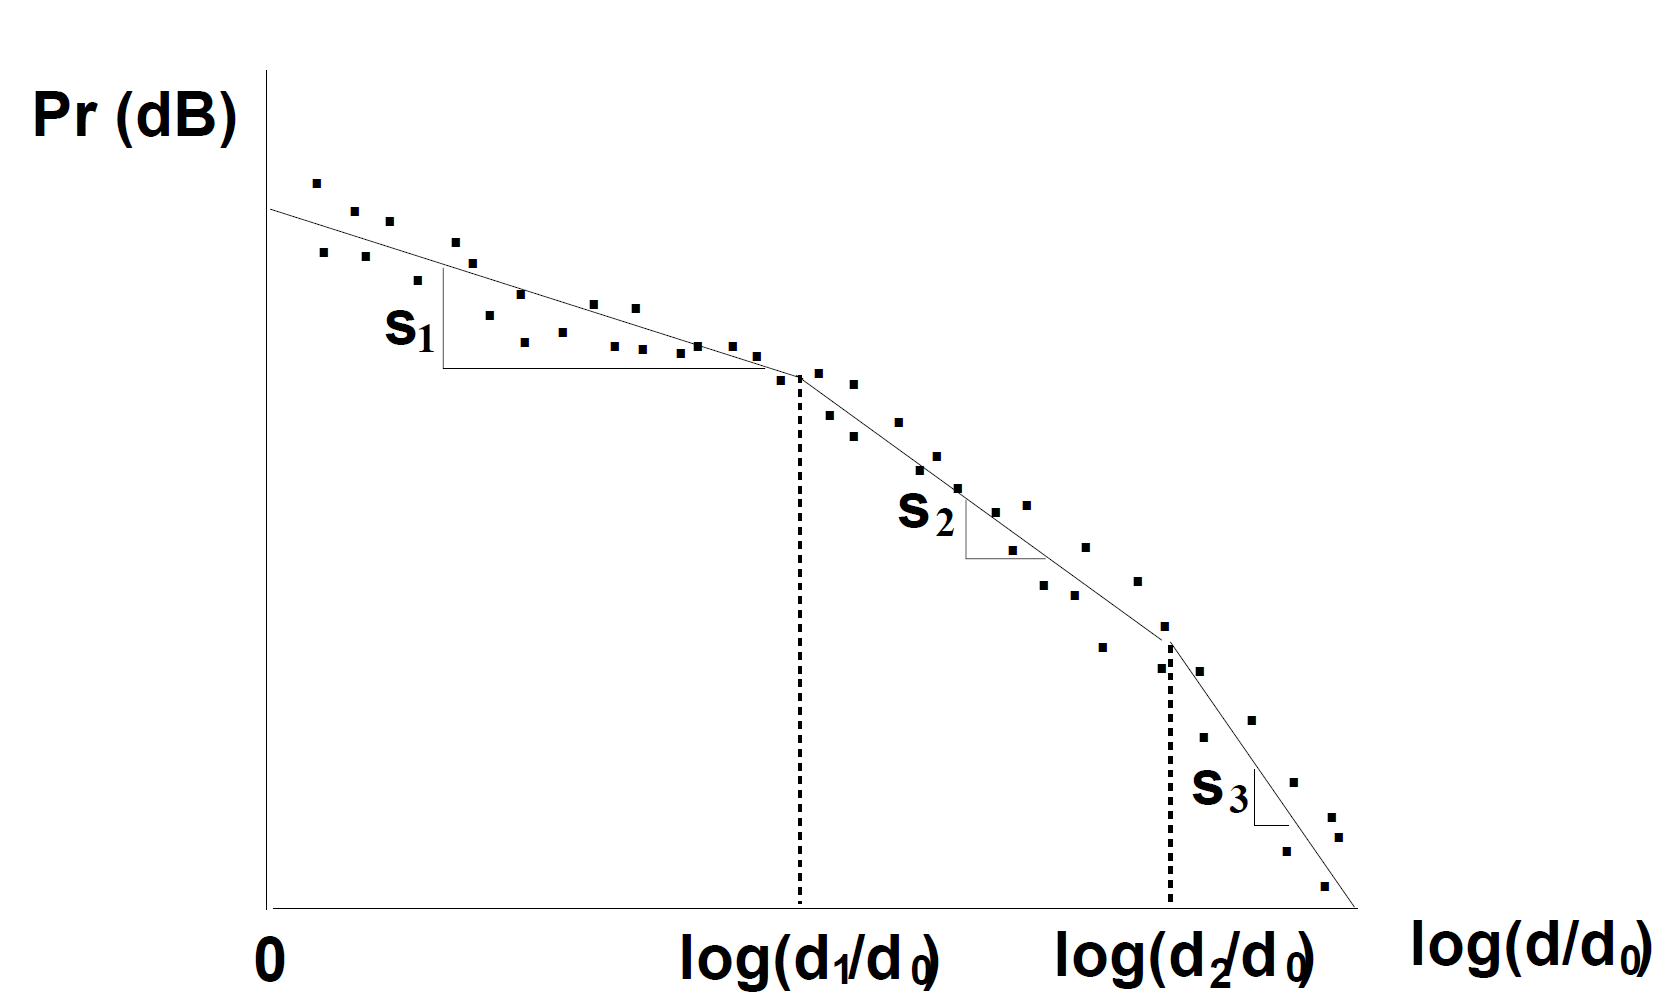
\includegraphics[width=0.8\textwidth]{fig/fig9.png}
		\caption{Piecewise Linear Model for Path Loss.}
		\label{fig:piecewise_linear_model}
	\end{figure}
	
	En specialtilfælde af den stykvis lineære model er \textit{dual-slope} modellen. \textit{Dual-slope} modellen er karakteriseret ved en konstant \textit{path loss factor} \(K\) og en \textit{path loss} eksponent \( \gamma_1 \) over en referenceafstand \( d_0 \) op til en kritisk afstand \( d_c \), hvorefter signalet falder med \textit{path loss} eksponenten \( \gamma_2 \):
	
	\[
	P_r(d) \, \text{dB} = 
	\begin{cases} 
		P_t + K - 10 \gamma_1 \log_{10}(d/d_0) & \text{for } d_0 \leq d \leq d_c \\
		P_t + K - 10 \gamma_1 \log_{10}(d_c/d_0) - 10 \gamma_2 \log_{10}(d/d_c) & \text{for } d > d_c 
	\end{cases}
	\]
	
	Her er \(P_t\) transmitterens effekt, \(P_r(d)\) den modtagne effekt som funktion af afstanden, og \(\gamma_1\) samt \(\gamma_2\) er \textit{path loss} eksponenter, der typisk opnås via regression af empiriske data.
	\newline\newline
	De multiple ligninger i \textit{dual-slope} modellen kan samles i følgende \textit{dual-slope} approximation:
	
	\[
	P_r = \frac{P_t K}{L(d)}
	\]
	
	hvor
	
	\[
	L(d) \triangleq \left(\frac{d}{d_0}\right)^{\gamma_1} \sqrt{1 + \left(\frac{d}{d_c}\right)^{(\gamma_1 - \gamma_2)q}}
	\]
	
	I dette udtryk er \(q\) en parameter, der bestemmer smoothness af \textit{path loss} ved overgangsområdet tæt på brudpunktet \(d_c\). Denne model kan udvides til mere end to regioner, hvis det er nødvendigt.
	\newline\newline
	Denne stykvis lineære model giver en fleksibel metode til at modellere \textit{path loss} over et bredt spektrum af afstande og anvendes ofte i både udendørs og indendørs kanaler.
	
	
	\subsection{Indendørs Attenuation Faktorer}
	Indendørs path loss modeller er essentielle for at forudsige signalstyrke inde i bygninger, hvor signalet møder forskellige hindringer som vægge, gulve og møbler. Tabellen nedenfor viser typiske attenuationer for forskellige materialer:
	
	\begin{table}[h]
		\centering
		\begin{tabular}{|l|c|}
			\hline
			\textbf{Materiale} & \textbf{Attenuation (dB)} \\
			\hline
			Tøj & 1.4 \\
			Dobbelt gipsvæg & 3.4 \\
			Foilisolering & 3.9 \\
			Betonvæg & 13 \\
			Aluminiumskonstruktion & 20.4 \\
			Alt Metal & 26 \\
			\hline
		\end{tabular}
		\caption{Typiske partitionstab for indendørs omgivelser.}
	\end{table}
	
	Disse data anvendes i formlen:
	
	\[
	P_r \, \text{dBm} = P_t \, \text{dBm} - P_L(d) - \sum_{i=1}^{N_f} FAF_i - \sum_{i=1}^{N_p} PAF_i
	\]
	
	Hvor:
	\begin{itemize}
		\item \( FAF_i \) er floor attenuation factor for den \( i \)te etage,
		\item \( PAF_i \) er partition attenuation factor for den \( i \)te skillevæg.
	\end{itemize}
	
	\noindent 
	Disse faktorer er essentielle for at beregne præcis signalstyrke inde i bygninger, hvor hver etage eller væg bidrager til det samlede path loss.
	
	
	\section{Simplified Path Loss Model}
	Når vi arbejder med trådløs kommunikation, er det vigtigt at kunne forudsige, hvordan signalstyrken ændrer sig, når afstanden mellem sender og modtager øges. Dette kaldes ofte for \textit{path loss}, og det beskriver, hvor meget af signalets styrke der går tabt på vej til modtageren.
	\newline\newline
	Der findes mange modeller, der kan bruges til at forudsige \textit{path loss}, men ofte kan en simpel model være tilstrækkelig til at give os en god forståelse af, hvad der sker. En af disse enkle modeller beskriver forholdet mellem modtagen effekt \( P_r \) og senderens effekt \( P_t \) som:
	
	\[
	P_r = P_t K \left[\frac{d_0}{d}\right]^\gamma
	\]
	
	\noindent hvor:
	
	- \( P_r \) er den modtagne effekt ved modtageren.
	- \( P_t \) er den effekt, der sendes fra senderen.
	- \( K \) er en konstant, som afhænger af antennens egenskaber og det gennemsnitlige signaltab i kanalen.
	- \( d_0 \) er en referenceafstand, typisk valgt i nærheden af senderen, hvor signalet stadig er stærkt.
	- \( d \) er afstanden mellem sender og modtager.
	- \( \gamma \) er \textit{path loss} eksponenten, som beskriver, hvor hurtigt signalet mister styrke over afstand.
	\newline\newline
	Denne model viser, at signalet bliver svagere, jo længere væk modtageren er fra senderen. Konstanten \( K \) kan beregnes ved hjælp af følgende formel, hvor \( \lambda \) er signalets bølgelængde:
	
	\[
	K \, \text{dB} = 20 \log_{10} \left(\frac{\lambda}{4\pi d_0}\right)
	\]
	
	\noindent Dette udtryk bruger vi, når vi ønsker at finde ud af, hvor meget signalstyrken falder ved en bestemt afstand \( d \) fra senderen.
	
	\subsection{Eksempel 1: Beregning af Path Loss Eksponent og Modtaget Effekt}
	\textbf{Problem:} Vi har et sæt empiriske målinger af forholdet mellem modtagen og sendt effekt \( P_r/P_t \) ved 900 MHz, som vist i tabellen nedenfor. Vi skal finde den \textit{path loss} eksponent \( \gamma \), der minimerer middelkvadratfejlen (MSE) mellem den simplificerede model (ligning 2.40) og de empiriske dB målinger, idet vi antager, at \( d_0 = 1 \) meter og \( K \) er bestemt ud fra \textit{free space path loss} formlen ved denne afstand. Dernæst skal vi beregne den modtagne effekt ved 150 meter for den simplificerede \textit{path loss} model med denne \( \gamma \) og en sendeeffekt på 1 mW (0 dBm).
	
	\begin{table}[h]
		\centering
		\begin{tabular}{|c|c|}
			\hline
			Afstand fra Transmitter (m) & \( M = P_r/P_t \) \\
			\hline
			10 m & -70 dB \\
			20 m & -75 dB \\
			50 m & -90 dB \\
			100 m & -110 dB \\
			300 m & -125 dB \\
			\hline
		\end{tabular}
		\caption{Path Loss målinger}
	\end{table}
	
	\noindent\textbf{Løsning:} Vi opstiller først MSE-fejludtrykket for dB målingerne som:
	
	\[
	F(\gamma) = \sum_{i=1}^{5} \left[ M_{\text{measured}}(d_i) - M_{\text{model}}(d_i) \right]^2
	\]
	
	hvor \( M_{\text{measured}}(d_i) \) er path loss målingen fra tabel 2.3 ved afstand \( d_i \), og \( M_{\text{model}}(d_i) \) er path loss baseret på (2.40) ved \( d_i \). Ved brug af formlen for \textit{free space path loss}, \( K = 20 \log_{10}(0.3333/(4\pi)) = -31.54 \) dB, får vi:
	
	\[
	F(\gamma) = (-70 + 31.54 + 10\gamma \log_{10}(10))^2 + (-75 + 31.54 + 13.01\gamma)^2 + (-90 + 31.54 + 16.99\gamma)^2 
	\]
	\[
	+ (-110 + 31.54 + 20\gamma)^2 + (-125 + 31.54 + 24.77\gamma)^2 
	\]
	\[
	F(\gamma) = 21676.3 - 11654.9\gamma + 1571.47\gamma^2
	\]
	
	\noindent Ved at differentiere \( F(\gamma) \) med hensyn til \( \gamma \) og sætte det lig nul, får vi:
	
	\[
	\frac{\partial F(\gamma)}{\partial \gamma} = -11654.9 + 3142.94\gamma = 0 \Rightarrow \gamma = 3.71
	\]
	
	For at finde den modtagne effekt ved 150 meter under den simplificerede \textit{path loss} model med \( K = -31.54 \) dB, \( \gamma = 3.71 \), og \( P_t = 0 \) dBm, har vi:
	
	\[
	P_r = P_t + K - 10\gamma \log_{10}(d/d_0) = 0 - 31.54 - 10 \times 3.71 \log_{10}(150/1) 
	\]
	\[
	P_r = -31.54 - 10 \times 3.71 \times 2.176 = -31.54 - 80.58 = -112.12 \text{ dBm}
	\]
	
	\noindent Denne afvigelse fra den simplificerede \textit{path loss} model kan tilskrives \textit{shadow fading}, som er beskrevet i Sektion 2.7.
	
	\subsection{Eksempel 2: Beregning af Modtaget Effekt ved 200 meter}
	\textbf{Problem:} Vi ønsker at beregne den modtagne effekt ved en afstand på 200 meter fra senderen, hvor den sendte effekt \( P_t \) er 1 mW (0 dBm), og \( \gamma = 3.71 \) er bestemt fra det foregående eksempel.
	\newline\newline\noindent
	\textbf{Løsning:} Vi anvender den samme formling som tidligere:
	
	\[
	P_r = P_t + K - 10\gamma \log_{10}(d/d_0)
	\]
	
	\[
	P_r = 0 \text{ dBm} - 31.54 - 10 \times 3.71 \log_{10}(200/1)
	\]
	
	\[
	P_r = -31.54 - 10 \times 3.71 \times 2.301 = -31.54 - 85.41 = -116.95 \text{ dBm}
	\]
	
	\textbf{Resultat:} Den modtagne effekt ved 200 meters afstand er cirka -116.95 dBm.
	
	\subsection{Eksempel 3: Effekt af \textit{Shadow Fading}}
	
	\textbf{Problem:} Antag, at vi har en situation, hvor \textit{shadow fading} introducerer en ekstra dæmpning på 10 dB ved en afstand på 100 meter. Beregn den samlede modtagne effekt under disse forhold.
	\newline\newline\noindent
	\textbf{Løsning:} Først beregner vi den modtagne effekt uden \textit{shadow fading}:
	
	\[
	P_r = 0 \text{ dBm} - 31.54 - 10 \times 3.71 \log_{10}(100/1)
	\]
	
	\[
	P_r = -31.54 - 10 \times 3.71 \times 2 = -31.54 - 74.2 = -105.74 \text{ dBm}
	\]
	
	Dernæst tager vi \textit{shadow fading} i betragtning:
	
	\[
	P_r = -105.74 \text{ dBm} - 10 \text{ dB} = -115.74 \text{ dBm}
	\]
	\noindent\textbf{Resultat:} Den samlede modtagne effekt ved 100 meter afstand, inklusive \textit{shadow fading}, er cirka -115.74 dBm.
	
	
	\subsection{Opsummering}
	
	Disse eksempler viser, hvordan vi kan bruge den simplificerede \textit{path loss} model til at beregne signalstyrken ved forskellige afstande i forskellige miljøer. Modellen gør det muligt at forudsige, hvor meget signalstyrken vil falde, og dermed hjælpe med at designe mere effektive trådløse netværk.
	
	
	\section{Shadow Fading og Log-Normal Skjulte Variabler}
	
	I trådløs kommunikation oplever signaler ofte variationer i modtaget effekt på grund af forhindringer som bygninger, træer eller andre objekter, der blokerer signalets vej. Denne tilfældige variation i signalstyrken kaldes \textit{shadow fading} eller log-normal fading, og det kan føre til væsentlige udsving i signalkvaliteten. For at modellere denne variation benyttes ofte en statistisk model kendt som log-normal fading model, som beskriver signalets dæmpning over afstand i en given kanal.
	
	\subsection{Log-Normal Skjulte Variabler}
	
	I log-normal fading-modellen antages det, at forholdet mellem den transmitterede effekt \( P_t \) og den modtagne effekt \( P_r \) er en tilfældig variabel \( \psi = \frac{P_t}{P_r} \), som er log-normalt fordelt. Dette betyder, at \( \log_{10}(\psi) \) er normalfordelt, hvilket kan udtrykkes som:
	
	\[
	p(\psi) = \frac{\xi}{\sqrt{2\pi\sigma_{\psi\text{dB}}^2}} \exp \left[ -\frac{(\log_{10}\psi - \mu_{\psi\text{dB}})^2}{2\sigma_{\psi\text{dB}}^2} \right], \quad \psi > 0
	\]
	
	hvor \( \xi = \frac{10}{\ln 10} \), \( \mu_{\psi\text{dB}} \) er middelværdien af \( \log_{10}(\psi) \) i dB, og \( \sigma_{\psi\text{dB}} \) er standardafvigelsen af \( \log_{10}(\psi) \) i dB.
	
	\subsection{Gennemsnit og Varians af \( \log_{10}(\psi) \)}
	
	Det er vigtigt at bemærke, at hvis \( \psi \) er log-normal, vil gennemsnittet og standardafvigelsen af \( \log_{10}(\psi) \) også være log-normale. Det betyder, at både modtagerens signal-til-støj-forhold (SNR) og modtagerens effekt vil være log-normale størrelser. Middelværdien \( \mu_\psi \) og standardafvigelsen \( \sigma_\psi \) for den modtagne effekt i dB kan findes ved:
	
	\[
	\mu_\psi = \mathbb{E}[\psi] = \exp \left[ \mu_{\psi\text{dB}} + \frac{\sigma_{\psi\text{dB}}^2}{2\xi^2} \right]
	\]
	
	Og konverteringen fra lineær middelværdi til log-middelværdi er givet ved:
	
	\[
	10 \log_{10} \mu_\psi = \mu_{\psi\text{dB}} + \frac{\sigma_{\psi\text{dB}}^2}{2\xi^2}
	\]
	
	\subsection{Shadow Fading Modellering}
	
	Modelleringen af shadow fading indebærer at finde middelværdi og varians af \( \psi \) for at forstå, hvordan modtaget effekt varierer i forskellige miljøer. Typisk er standardafvigelsen \( \sigma_{\psi\text{dB}} \) i området fra 4 til 13 dB, afhængigt af miljøet. For eksempel vil urban macrocells have en højere standardafvigelse på grund af flere forhindringer end åbne områder.
	
	En vigtig del af denne model er at forudsige signalstyrken \( s(d) \) som en funktion af afstanden \( d \) fra senderen:
	
	\[
	s(d) = e^{-\alpha d}
	\]
	
	hvor \( \alpha \) er en dæmpningskonstant, der afhænger af objekternes materialer og dielektriske egenskaber. Når signalet passerer gennem flere objekter, vil den samlede dæmpning \( s(d) \) være:
	
	\[
	s(d_t) = e^{-\alpha \sum d_i} = e^{-\alpha d_t}
	\]
	
	hvor \( d_t \) er summen af dybderne af alle objekterne mellem senderen og modtageren.
	
	\subsection{Eksempler}
	
	\subsubsection{Eksempel 2.4: Beregning af Shadow Fading Varians}
	
	Givet en række målinger af \( \frac{P_r}{P_t} \) fra et indendørs system ved 900 MHz, beregn variansen \( \sigma_{\psi\text{dB}}^2 \) for shadow fading over en given afstand.
	
	\begin{enumerate}
		\item \textbf{Dataanalyse}: Vi tager fem målepunkter fra tabel 2.3, der giver os \( M_{\text{measured}}(d_i) \) og \( M_{\text{model}}(d_i) \).
		\item \textbf{Fejlberegning}: Vi beregner fejlens kvadratrod ved hver afstand ved at sammenligne den målte effekt med den beregnede model.
		\item \textbf{Variansberegning}:
		\[
		\sigma_{\psi\text{dB}}^2 = \frac{1}{5} \sum_{i=1}^{5} \left[ M_{\text{measured}}(d_i) - M_{\text{model}}(d_i) \right]^2
		\]
		\item \textbf{Resultat}: Vi finder \( \sigma_{\psi\text{dB}} = 3.65 \) dB, hvilket er standardafvigelsen for shadow fading i dette miljø.
	\end{enumerate}
	
	\subsubsection{Eksempel 2.5: Beregning af Skjulte Variabler i Et Byområde}
	
	Antag en frekvens på 2 GHz i et byområde med høje bygninger. Beregn den gennemsnitlige effekt \( \mu_{\psi\text{dB}} \) for modtageren placeret 100 meter væk fra senderen.
	
	\begin{enumerate}
		\item \textbf{Middelværdi i dB}:
		\[
		\mu_{\psi\text{dB}} = \exp \left[ \mu_{\psi\text{dB}} + \frac{\sigma_{\psi\text{dB}}^2}{2\xi^2} \right]
		\]
		\item \textbf{Standardafvigelse}: Antag \( \sigma_{\psi\text{dB}} = 8 \) dB, og brug de tidligere angivne data til at beregne den gennemsnitlige modtagne effekt.
		\item \textbf{Resultat}: Den modtagne effekt er reduceret betydeligt på grund af shadow fading, især i byområder.
	\end{enumerate}
	
	\subsubsection{Eksempel 2.6: Anvendelse af Shadow Fading i Et Mikrocellulært Miljø}
	
	Beregning af signalstyrken for et mikrocellesystem ved 2 GHz, hvor modtageren er placeret 50 meter væk fra senderen, og der er flere forhindringer som træer og bygninger.
	
	\begin{enumerate}
		\item \textbf{Dæmpningskonstant}:
		\[
		\alpha = \frac{\sigma_{\psi\text{dB}}}{\sqrt{2}}
		\]
		\item \textbf{Beregn signalstyrken}:
		\[
		s(d) = e^{-\alpha d}
		\]
		\item \textbf{Resultat}: Variationen i signalstyrken afhænger af antallet og størrelsen af forhindringerne mellem senderen og modtageren.
	\end{enumerate}
	
	Disse eksempler hjælper med at forstå, hvordan shadow fading påvirker signaludbredelsen i forskellige miljøer og hvordan det kan modelleres for at optimere trådløse kommunikationssystemer.
	
	\section{Combined Path Loss and Shadowing}
	Modeller for path loss og shadowing kan kombineres for at fange både effekten af signalstyrketab over afstand samt tilfældig attenuation, der skyldes shadowing. I denne kombinerede model bliver det gennemsnitlige dB path loss karakteriseret af path loss-modellen, mens shadow fading med en middelværdi på 0 dB skaber variationer omkring dette path loss, som illustreret af kurven i figur 2.1. Specifikt plotter denne kurve kombinationen af den forenklede path loss-model (ligning 2.39) og den log-normal shadowing tilfældige proces defineret af ligningerne (2.46) og (2.50). For denne kombinerede model er forholdet mellem modtaget og transmitteret effekt i dB givet ved:
	
	\[
	\frac{P_r}{P_t} \text{(dB)} = 10 \log_{10} K - 10 \gamma \log_{10}\left(\frac{d}{d_0}\right) - \psi_{\text{dB}},
	\]
	\noindent hvor \( \psi_{\text{dB}} \) er en Gauss-fordelt tilfældig variabel med middelværdien nul og variansen \( \sigma^2_{\psi_{\text{dB}}} \). I ligning (2.51) og som vist i figur 2.1, falder path loss lineært i forhold til \( \log_{10}(d) \) med en hældning på \( 10 \gamma \) dB per dekade, hvor \( \gamma \) er path loss eksponenten. Variationer som følge af shadowing ændrer sig hurtigere, afhængig af decorrelation distance \( X_c \).
	
	De foregående eksempler 2.3 og 2.4 illustrerer den kombinerede model for path loss og log-normal shadowing baseret på målingerne i tabel 2.3, hvor path loss følger den forenklede model med \( K = -31.54 \) dB og path loss eksponenten \( \gamma = 3.71 \), mens shadowing følger log-normal modellen med middelværdi givet af path loss modellen og standardafvigelsen \( \sigma_{\psi_{\text{dB}}} = 3.65 \) dB.
	
	\subsection{Statistisk Baggrund for Shadowing}
	Shadowing refererer til de tilfældige udsving i signalstyrken, som skyldes blokeringer eller forhindringer i signalets vej, som kan være forårsaget af bygninger, træer eller andre objekter. Disse udsving modelleres ofte som en log-normal fordeling, hvor \( \psi_{\text{dB}} \) beskriver forskellen mellem den forventede signalstyrke og den faktiske målte styrke.
	
	Den log-normale fordeling er kendetegnet ved, at hvis \( \psi \) i sig selv varierer over en bred vifte, så vil \( \log_{10}(\psi) \) være normalfordelt. Dette gør det muligt at bruge standardstatistiske metoder til at analysere dataene. Den normalfordelte tilfældige variabel \( \psi_{\text{dB}} \) har en middelværdi på nul og en varians \( \sigma^2_{\psi_{\text{dB}}} \), hvilket beskriver spredningen af shadowing-effekten omkring det gennemsnitlige path loss.
	\newline\newline
	For at beregne den samlede effekt af path loss og shadowing, kan man bruge ligning (2.51) ovenfor, hvor \( \psi_{\text{dB}} \) repræsenterer den tilfældige variation, der skyldes shadowing.
	
%	\begin{figure}[h]
%		\centering
%		\includegraphics[width=0.8\textwidth]{path_loss_and_shadowing_curve.png}
%		\caption{Kurven viser kombinationen af path loss og shadowing-effekter over afstand.}
%	\end{figure}
	
	Denne kombination af path loss og shadowing giver os en mere realistisk model for signaludbredelse i komplekse miljøer, hvor både systematiske og tilfældige effekter spiller en rolle.
	
	\section{Outage Probability under Path Loss and Shadowing}
	
	De kombinerede effekter af path loss og shadowing har vigtige implikationer for design af trådløse systemer. I trådløse systemer er der typisk et mål for den minimale modtagne effekt, \( P_{\text{min}} \), under hvilken ydeevnen bliver uacceptabel (f.eks. når lydkvaliteten i et mobilsystem er for dårlig til at forstå). Med shadowing kan den modtagne effekt på enhver given afstand fra senderen variere log-normalt med en vis sandsynlighed for at falde under \( P_{\text{min}} \).
	
	Vi definerer \textit{outage probability} \( p_{\text{out}}(P_{\text{min}}, d) \) under path loss og shadowing som sandsynligheden for, at den modtagne effekt på en given afstand \( d \), \( P_r(d) \), falder under \( P_{\text{min}} \). Det vil sige:
	
	\[
	p(P_r(d) \leq P_{\text{min}}) = 1 - Q\left(\frac{P_{\text{min}} - \left(P_t + 10 \log_{10} K - 10 \gamma \log_{10}(d/d_0)\right)}{\sigma_{\psi_{\text{dB}}}}\right),
	\]
	
	hvor \( Q(z) \)-funktionen defineres som sandsynligheden for, at en Gauss-fordelt tilfældig variabel \( x \) med middelværdien nul og variansen ét er større end \( z \). 
	
	\[
	Q(z) \triangleq p(x > z) = \int_{z}^{\infty} \frac{1}{\sqrt{2\pi}} e^{-y^2/2} dy.
	\]
	
	For nemhedens skyld benytter vi ofte den komplementære fejl-funktion, som er relateret til \( Q \)-funktionen:
	
	\[
	Q(z) = \frac{1}{2} \text{erfc}\left(\frac{z}{\sqrt{2}}\right).
	\]
	
	\subsection{Eksempel 2.5: Beregning af Outage Probability}
	\noindent Lad os finde \textit{outage probability} ved en afstand på 150 meter for en kanal baseret på de kombinerede path loss og shadowing-modeller fra Eksempel 2.3 og 2.4. Vi antager en sendereffekt på \( P_t = 10 \) mW og et minimum effektkrav \( P_{\text{min}} = -110.5 \) dBm.
	
	\subsubsection*{Løsning:}
	Vi har \( P_t = 10 \) mW = 10 dBm. 
	
	\[
	P_{\text{out}}(-110.5 \text{dBm}, 150 \text{m}) = p(P_r(150 \text{m}) < -110.5 \text{dBm})
	\]
	
	\[
	= 1 - Q\left(\frac{P_{\text{min}} - \left(P_t + 10 \log_{10} K - 10 \gamma \log_{10}(d/d_0)\right)}{\sigma_{\psi_{\text{dB}}}}\right)
	\]
	
	\[
	= 1 - Q\left(\frac{-110.5 - (10 - 31.54 - 37.1 \log_{10}(150))}{3.65}\right)
	\]
	
	\[
	= 1 - Q\left(\frac{-110.5 - (-131.41)}{3.65}\right)
	\]
	
	\[
	= 1 - Q\left(\frac{20.91}{3.65}\right)
	\]
	
	\[
	= 1 - Q(5.73) \approx 0.0121.
	\]
	
	\noindent En \textit{outage probability} på 1\% er typisk målet i design af trådløse systemer.
	
	\subsection{Statistisk Baggrund: Q-funktionen og Outage Probability}
	Q-funktionen er en standard funktion, der anvendes i statistikken til at beskrive sandsynligheden for, at en standard normalfordelt variabel overstiger en bestemt værdi. Dette er relevant i trådløse systemer, fordi variationerne i modtaget effekt ofte kan modelleres som log-normalfordelt, hvilket betyder, at de tilsvarende variationer i dB er normalfordelte. Når vi beregner \textit{outage probability}, bruger vi Q-funktionen til at bestemme sandsynligheden for, at den modtagne effekt falder under en vis tærskel.
	\newline\newline
	Denne metode er særlig vigtig i systemdesign, da den hjælper os med at forstå og sikre, at systemet fungerer tilfredsstillende selv i tilstedeværelse af tilfældige variationer som følge af shadowing.
	
	\section{Cell Coverage Area}
	\label{sec:cell_coverage}
	
	Cell coverage area i et cellulært system refererer til den procentdel af området inden for en celle, hvor den modtagne effekt er tilstrækkelig til at opfylde systemets krav til ydeevne. For at forstå dette koncept bedre, lad os overveje en basestation (BS), der er placeret centralt i en cirkulær celle med en radius \( R \).
	
	\subsection{Basestationens Rolle i Dækning}
	Basestationen transmitterer et signal med en effekt, der skal sikre, at den modtagne signalstyrke \( P_r \) på alle punkter i cellen er over en minimumsværdi \( P_{\text{min}} \), som er nødvendig for at opretholde en acceptabel ydeevne, f.eks. i form af en tilstrækkelig Signal-to-Noise Ratio (SNR). Dette krav gælder især ved cellegrænsen, hvor signalstyrken naturligt vil være svagest på grund af afstanden fra basestationen.
	
	\subsection{Effekten af Path Loss og Shadowing}
	Som tidligere nævnt påvirkes signalstyrken i cellen både af path loss (den systematiske reduktion i signalstyrke over afstand) og af shadowing (de tilfældige udsving i signalstyrken forårsaget af objekter i signalvejen). Disse effekter kombineres og resulterer i, at signalstyrken i praksis varierer betydeligt over celleområdet.
	
	\begin{figure}[h]
		\centering
		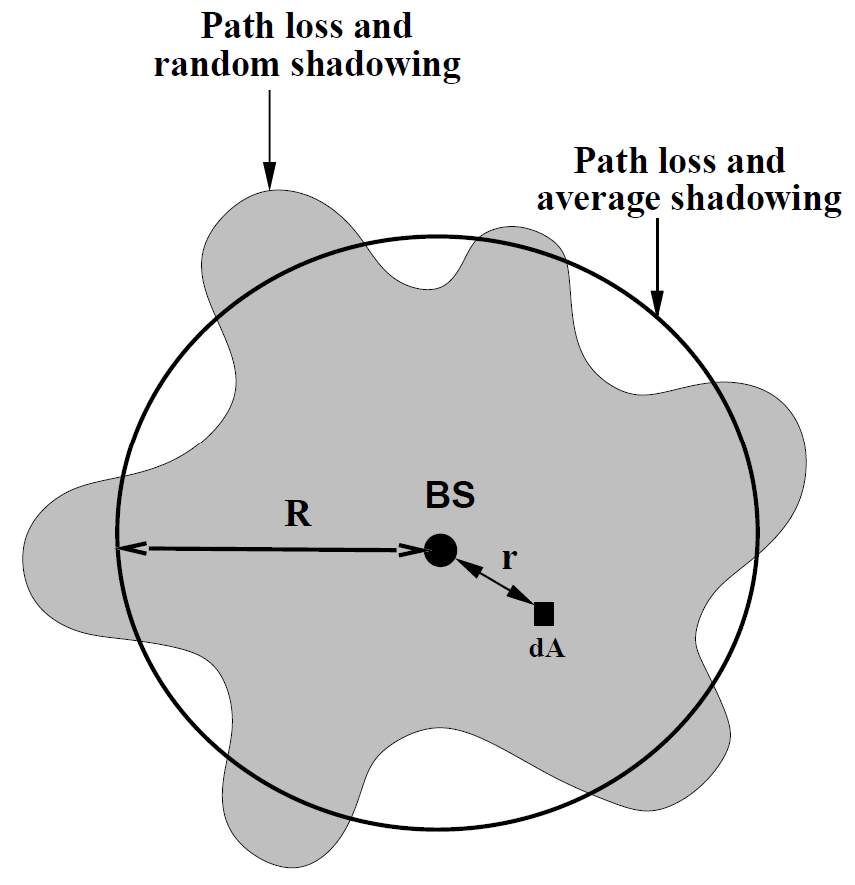
\includegraphics[width=0.4\textwidth]{fig/fig10.png}
		\caption{Illustration af cellulær dækning påvirket af path loss og shadowing. Figuren viser, hvordan shadowing resulterer i uregelmæssige konturer for modtaget signalstyrke i en cirkulær celle med radius \(R\).}
	\end{figure}
	\clearpage
	\subsection{Matematisk Modellering af Dækningen}
	Dækningen \( C \) i cellen defineres som det forventede areal, hvor den modtagne effekt \( P_r \) overstiger \( P_{\text{min}} \). Dette kan formelt beregnes ved at integrere over alle de områder \( dA \) i cellen, hvor dette krav er opfyldt:
	
	\[
	C = E\left[\frac{1}{\pi R^2} \int_{\text{cell area}} 1[P_r(r) > P_{\text{min}} \text{ in dA}] dA\right]
	\]
	
	I dette udtryk repræsenterer \( 1[\cdot] \) en indikatorfunktion, som er 1, når betingelsen indenfor klammen er sand, og ellers 0. Dette betyder, at vi kun tæller de områder med, hvor \( P_r(r) > P_{\text{min}} \). Da dækningen kan variere inden for cellen, er det nødvendigt at tage et gennemsnit (forventningsværdi) over hele cellens areal.
	
	\subsection{Outage Probability}
	Et beslægtet begreb er outage probability, som er den sandsynlighed, at den modtagne effekt \( P_r \) falder under \( P_{\text{min}} \) i et givet område af cellen. Dette kan udtrykkes som:
	
	\[
	p_{\text{out}}(P_{\text{min}}, r) = 1 - Q\left(\frac{P_{\text{min}} - \left(P_t + 10 \log_{10} K - 10 \gamma \log_{10}(r/d_0)\right)}{\sigma_{\psi_{\text{dB}}}}\right)
	\]
	
	Her er \( Q(\cdot) \) den komplementære fejlfunktion, som beregner sandsynligheden for, at en normalfordelt variabel overskrider en given værdi. Outage probability beskriver altså den del af celleområdet, hvor signalet ikke er stærkt nok til at sikre en pålidelig forbindelse.
	
	\subsection{Eksempler}
	
	\subsubsection{Eksempel 1: Beregning af Cell Coverage Area}
	
	Lad os antage, at vi har følgende parametre:
	\begin{itemize}
		\item Basestationens sendestyrke \( P_t = 100 \) mW (20 dBm)
		\item Modtagerens minimumskrav til signalstyrke \( P_{\text{min}} = -110 \) dBm
		\item Cellens radius \( R = 600 \) meter
		\item Path loss exponent \( \gamma = 3.71 \)
		\item Shadowing standard deviation \( \sigma_{\psi_{\text{dB}}} = 3.65 \) dB
	\end{itemize}
	
	Vi vil beregne dækningsområdet \( C \) ved brug af ligning (2.61):
	
	\[
	C = \frac{1}{2} + \frac{1}{2} \exp \left( \frac{2}{b^2} \right) Q \left( \frac{2}{b} \right),
	\]
	
	hvor \( a = \frac{P_{\text{min}} - P_R(R)}{\sigma_{\psi_{\text{dB}}}} \) og \( b = \frac{10 \gamma \log_{10}(e)}{\sigma_{\psi_{\text{dB}}}} \).
	
	\subsubsection{Eksempel 2: Beregning af Outage Probability}
	
	Antag, at vi ønsker at beregne outage probability for en bruger placeret 150 meter fra basestationen. Vi bruger følgende parametre:
	\begin{itemize}
		\item Basestationens sendestyrke \( P_t = 10 \) mW (10 dBm)
		\item Modtagerens minimumskrav til signalstyrke \( P_{\text{min}} = -110.5 \) dBm
		\item Afstand til basestationen \( d = 150 \) meter
		\item Path loss exponent \( \gamma = 3.71 \)
		\item Shadowing standard deviation \( \sigma_{\psi_{\text{dB}}} = 3.65 \) dB
	\end{itemize}
	
	Outage probability beregnes som:
	
	\[
	p_{\text{out}} = 1 - Q\left(\frac{-110.5 - \left(10 - 31.54 - 37.1 \log_{10}(150)\right)}{3.65}\right)
	\]
	
	\subsubsection{Eksempel 3: Beregning af Total Coverage Area}
	
	Hvis vi skal finde den totale dækningsgrad for cellen, hvor både path loss og shadowing er inkluderet, og vi har flere brugere jævnt fordelt i cellen, kan vi gentage beregningerne fra de tidligere eksempler for flere afstande og beregne gennemsnittet af disse resultater.
	
	\chapter{Opgaver}
	\section{Exercises week 2}
	
	\begin{enumerate}
		\item Under the free-space path loss model, find the transmit power required to obtain a received power of 1 dBm for a wireless system with isotropic antennas ($G_t = G_r = 1$) and a carrier frequency $f_c = 5$ GHz, assuming a distance $d = 10$ m. Repeat for $d = 100$ m.
		
		\item For the two-ray model with transmitter-receiver separation $d = 100$ m, $h_t = 10$ m, and $h_r = 2$ m, find the delay spread between the two signals.
		
		\item Find the critical distance $d_c$ under the two-ray model for a large macrocell in a suburban area with the base station mounted on a tower or building ($h_t = 20$ m), the receivers at height $h_r = 3$ m, and $f_c = 2$ GHz. Is this a good size for cell radius in a suburban macrocell? Why or why not?
		
		\item Consider a receiver with noise power $-160$ dBm within the signal bandwidth of interest. Assume a single-slope path loss model with $d_0 = 1$ m, $K$ obtained from the free-space path loss formula with isotropic antennas and $f_c = 1$ GHz, and $\gamma = 4$. For a transmit power of $P_t = 10$ mW, find the maximum distance between the transmitter and receiver such that the received signal-to-noise power ratio is 20 dB.
		
		\item Table 2.7 lists a set of empirical path loss measurements. Assume a carrier frequency $f_c = 2$ GHz.
		
		\begin{enumerate}
			\item Find the parameters of a single-slope path loss model plus log-normal shadowing that best fit this data assuming $K$ is calculated from free-space path loss at the reference distance $d_r = 1$ m.
			
			\item Find the path loss at 2 Km based on this model.
			
			\item Find the outage probability at a distance $d$ assuming the received power at $d$ due to path loss alone is 10 dB above the required power for non-outage.
		\end{enumerate}
	\end{enumerate}
	
	\begin{table}[h!]
		\centering
		\caption{Path loss measurements for Problem 2-14}
		\begin{tabular}{|c|c|}
			\hline
			\textbf{Distance from Transmitter} & $\mathbf{\frac{P_r}{P_t}}$ \\
			\hline
			5 m   & $-60$ dB \\
			25 m  & $-80$ dB \\
			65 m  & $-105$ dB \\
			110 m & $-115$ dB \\
			400 m & $-135$ dB \\
			1000 m & $-150$ dB \\
			\hline
		\end{tabular}
	\end{table}
	
\end{document}
